\chapter{Física del Modelo Estándar, y un poco más allá} \label{chap:ch1}

\begin{marginfigure}[27em]
    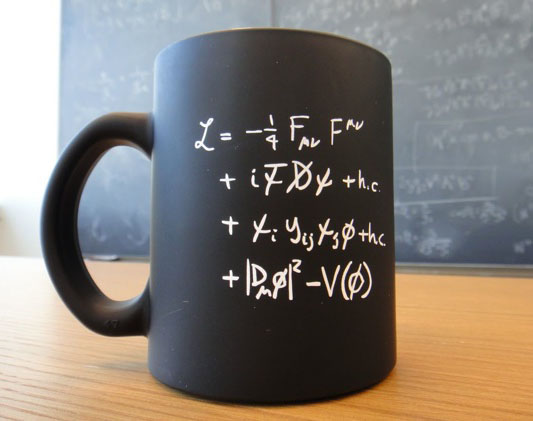
\includegraphics[width=0.99\linewidth]{Assets/Images/sm_mug.jpg}
    \caption{Lagrangiano contraído del SM, en un artículo de uso cotidiano por muchos físicos.}
    \label{fig:ch1:sm_mug}
\end{marginfigure}

\newthought{El Modelo Estándar}, o \textit{Standard Model} (SM), cuyo lagrangiano contraido podemos ver en la \cref{fig:ch1:sm_mug}, es la teoría más precisa y completa con la que contamos para describir las partículas elementales y sus interacciones. Iniciado por Glashow, Salam y Weinberg~\cite{Glashow1961,Weinberg1967,Salam1959} en la década de 1970 y cimentado en el marco de la Teoría Cuántica de Campos (QFT), las predicciones de está teoría han superado desafíos experimentales de alta precisión durante el siglo XX y XXI, culminando con el hallazgo del Bosón de Higgs en 2012 por el experimento ATLAS~\cite{TheATLASCollaboration2012} y CMS~\cite{TheCMSCollaboration2012}.

Sin embargo, el SM no puede ser considerado una teoría fundamental y completa: no incluye la gravedad (descrita por la Teoría de la Relatividad General); es excesivamente sensible a variaciones de algunos de sus parámetros; no incluye la masa de los neutrinos y no explica la naturaleza de la materia oscura, entre otros problemas. Para subsanar estas falencias, en los últimos 50 años se han propuesto vastas extensiones al Modelo Estándar, conocidos como modelos BSM (\textit{Beyond Standard Model}, más allá del Modelo Estándar). En particular, varias extensiones teóricas para el Modelo Estándar suponen la existencia de campos pseudoescalares (\textit{$CP$-odd}, impares ante transformaciones de conjugación de carga y paridad), en algunos casos extendiendo el sector escalar de Higgs.

En este capítulo daremos una breve introducción al Modelo Estándar, describiendo las partículas e interacciones que lo componen. Presentaremos brevemente los métodos efectivos que se utilizan para simular interacciones en un colisionador hadrónico, como el LHC. Luego, motivados principalmente por el problema de emisiones de rayos gamma difusos en los centros galácticos~\cite{Hooper2011}, desarrollaremos algunos modelos de extensión del SM que predicen la existencia de partículas pseudoescalares de masas inferiores a \SI{100}{\GeV}. En particular, nos enfocaremos en la producción de pseudoescalares en asociación a un par $t\bar{t}$, con un canal de decaimiento a 2 leptones tau.




\section{El Modelo Estándar}

El Modelo Estándar es una teoría cuántica de campos renormalizable, que describe las naturaleza de las partículas elementales y sus interacciones fuertes, débiles y electromagnéticas. Pese a describir solo el 5\% del universo observable -ya que desconocemos las propiedades de la materia y la energía orcura-, el SM es la teoría verificada experimentalmente más completa con la que contamos, con predicciones que acuerdan con los resultados experimentales en hasta 7.6 partes en $10^{13}$~\cite{Hanneke2008}.

El SM contempla la existencia de campos cuánticos, cuyas excitaciones son vinculadas con las partículas de materia (fermiones), los mediadores de las interacciones (bosones de gauge), y el bosón de Higgs. La materia se encuentra descrita por campos espinoriales (de spin $1/2$), mientras que los mediadores de las interacciones fuertes y electrodébiles se corresponden a bosones vectoriales (de spin $1$). El bosón de Higgs es el único campo escalar presente en el SM (con spin $0$).

Los fermiones son partículas de spin semientero, obedeciendo la estadística de Fermi-Dirac y encontrándose sujetas al principio de exclusión de Pauli. Pueden ser clasificados en dos grandes grupos: los leptones y los quarks, dependiendo si son portadores de carga de color que da lugar a la interacción fuerte. Más aún, como podemos observar en la \cref{fig:ch1:SM:particles} los fermiones del SM pueden organizarse en tres generaciones, compartiendo los mismos números cuánticos de spin y carga eléctrica, pero presentándose con diferente masa. La primera generación corresponde a las partículas más livianas, que constituyen la materia ordinaria (quarks up, down y electrones). Las partículas de la segunda y tercera generación no son estables y decaen luego de un corto período de tiempo a partículas de la primera generación. A excepción del quark top, en el régimen de bajas energías los quarks son solo observados en estados ligados conocidos como hadrones. Debido a su elevada masa, los quark top decaen rápidamente ($\tau \sim 10^{-25}\si{s}$), por lo que no tienen el tiempo necesario para hadronizar.

\begin{figure}[t]
  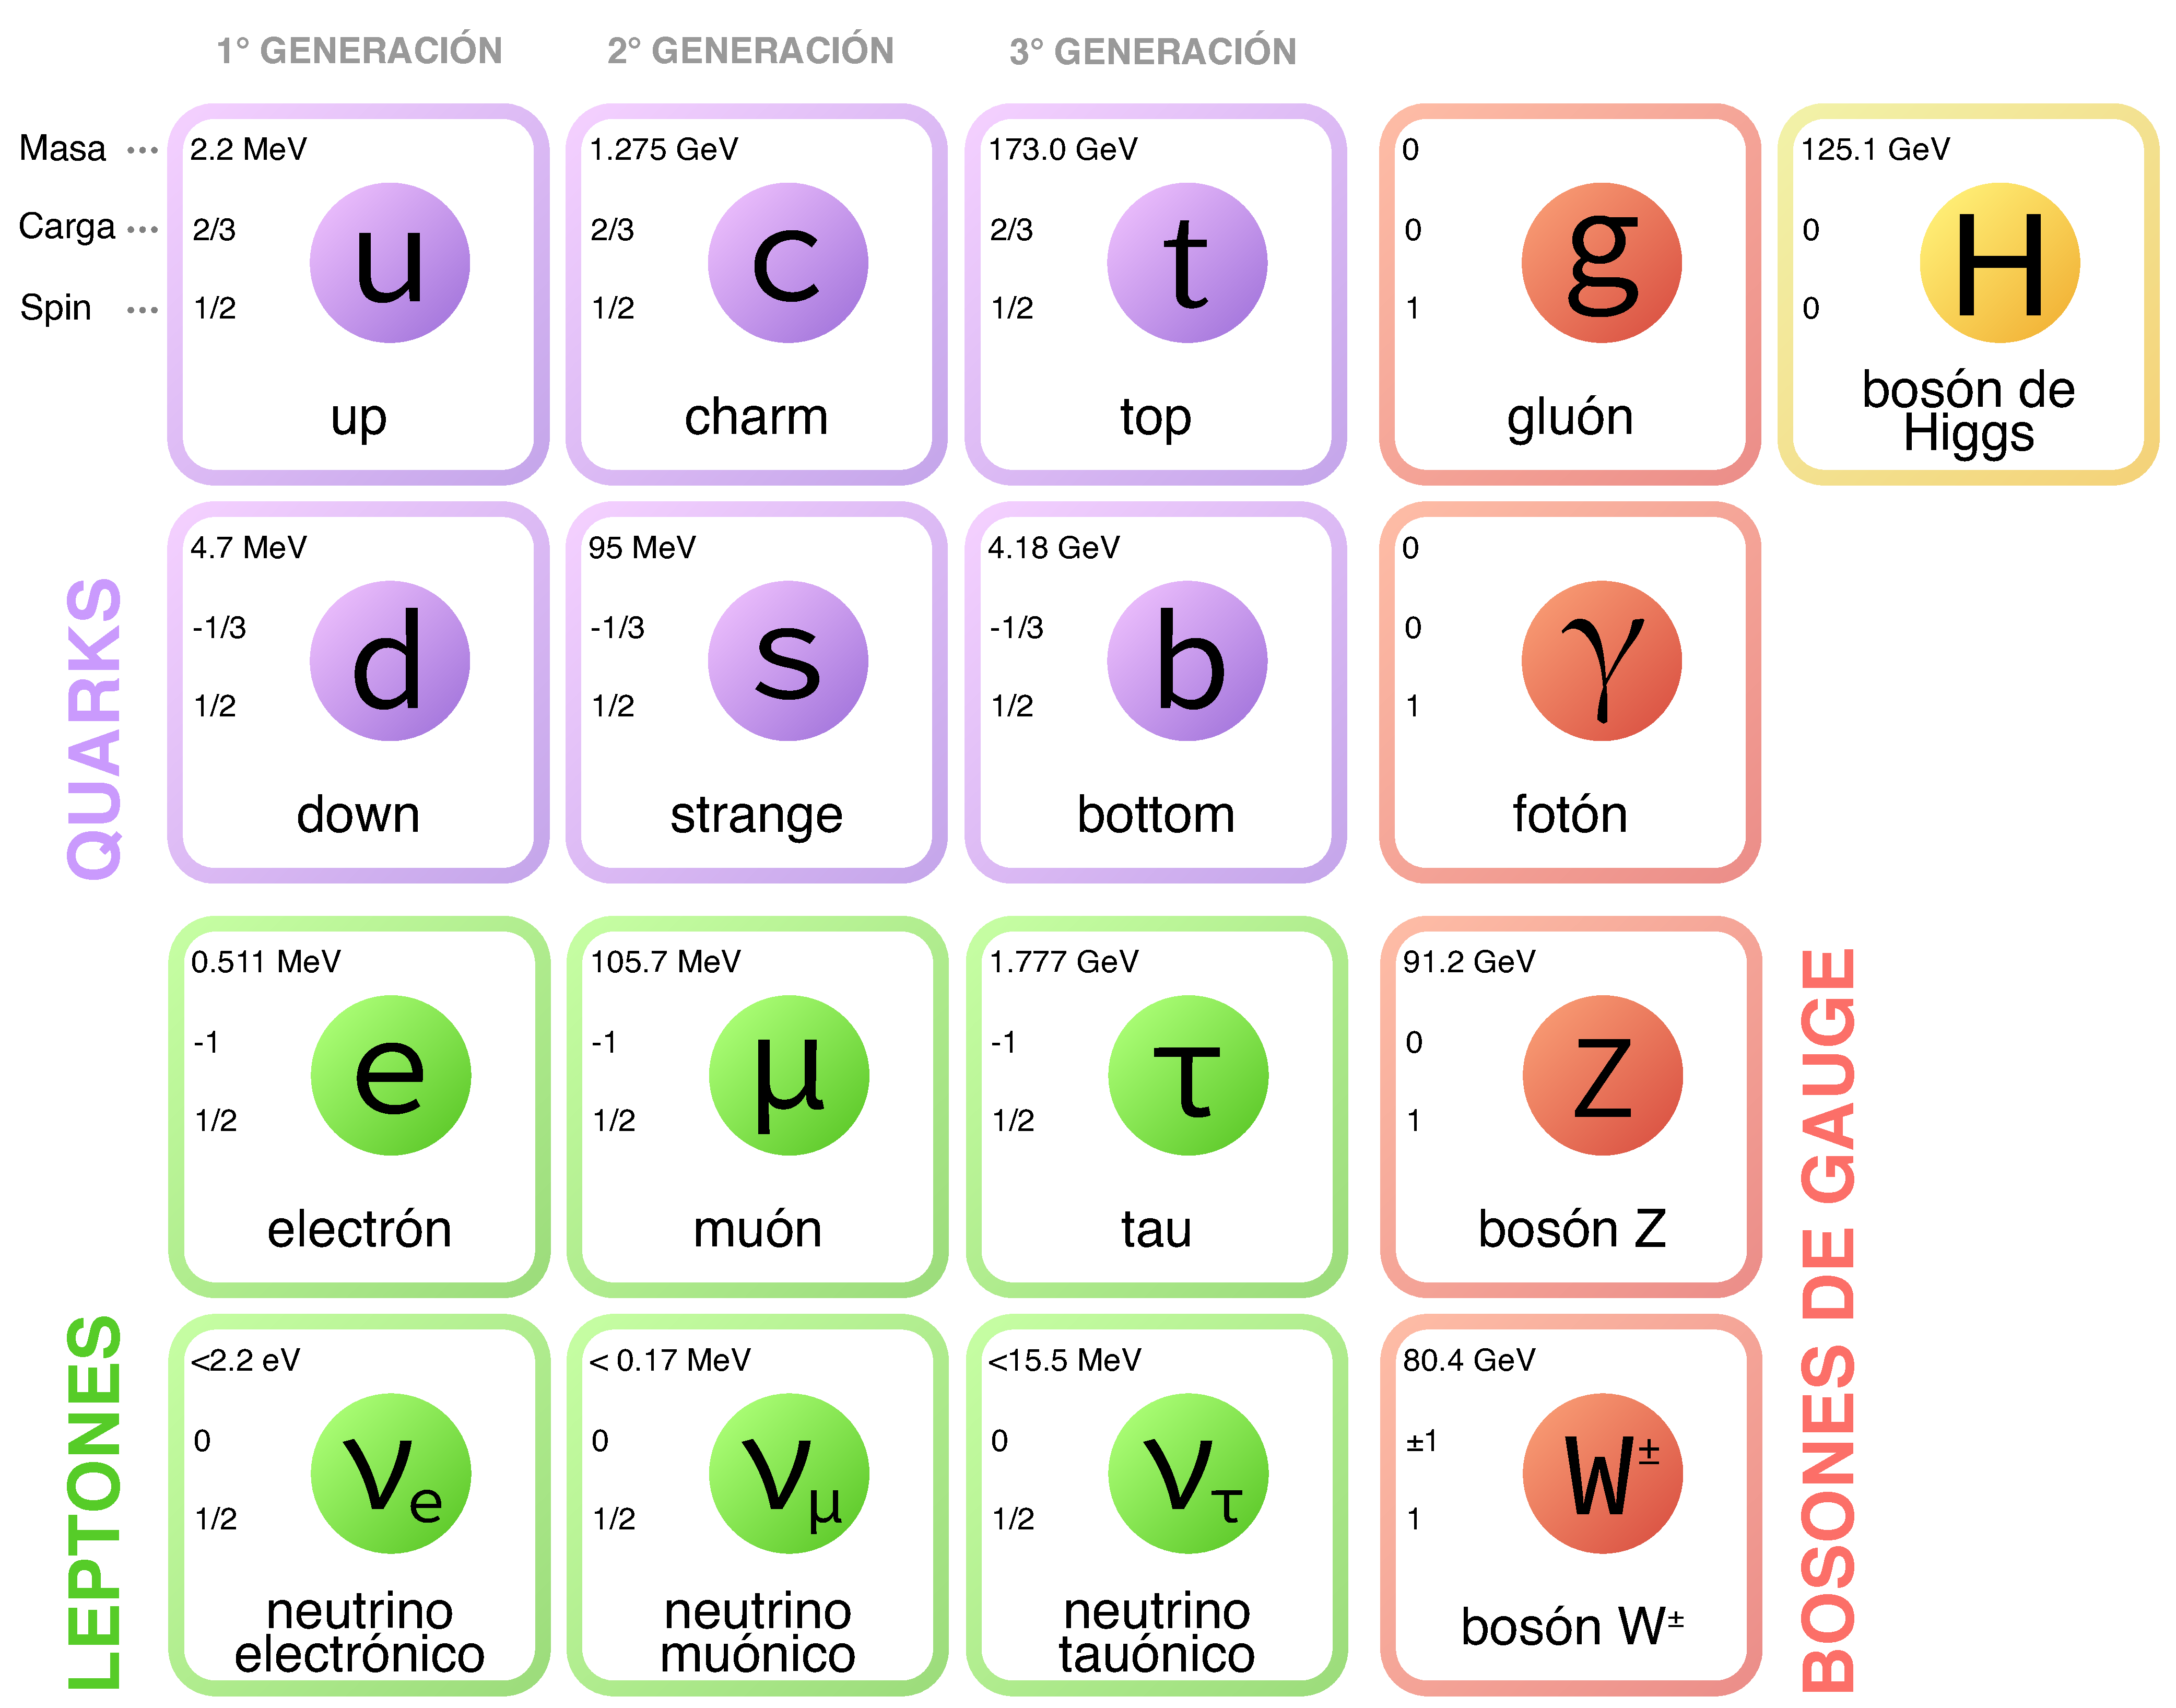
\includegraphics[width=\linewidth]{Assets/Images/Standard_model.pdf}
  \caption[Partículas que constituyen el Modelo Estándar][-2em]{Partículas que constituyen el Modelo Estándar, agrupadas en quarks, leptones, bosones de gauge y bosones escalares (el bosón de Higgs). Las masas de los neutrinos no son incluidas por el SM.}
  \label{fig:ch1:SM:particles}
  \setfloatalignment{b}
\end{figure}

En el caso de los leptones, cada generación se encuentra formada por una partícula cargada (electrones, muones y taus), de carga\sidenote{Por convención, expresamos la carga en unidades de la carga electrónica $e = \SI{1.602e-19}{\coulomb}$.} $q = -1$ y un neutrino neutro ($q = 0$). Por el contrario, todos los quarks poseen carga. Cada generación contiene un quark de tipo \textit{up}, con carga $+2/3$, y un quark de tipo \textit{down}, con carga $-1/3$. Para cada fermión de materia, la teoría cuántica relativista predice la existencia de una partícula de anti-materia, con la misma masa y spin, pero cargas y demás rótulos opuestos.

El SM es formulado como teoría de gauge no-abeliana, cuyo grupo de simetría de gauge está dado por el producto
\[ U(1)_Y \times SU(2)_L \times SU(3)_C. \]
El grupo no-abeliano $SU(3)_C$ de color describe las interacciones fuertes entre quarks y sus mediadores bosónicos, los gluones. Esta teoría es conocida como \textit{Cromodinámica Cuántica}. El sector electrodébil $SU(2)_L \times U(1)_Y$ es responsable de las interacciones débiles y electromagnéticas, luego de una ruptura espontánea de simetría $SU(2)_L \times U(1)_Y \to U(1)_{EM}$ producida por el potencial del bosón de Higgs. La interacción débil se encuentra mediada por tres bosones masivos, $W^\pm$ y $Z^0$, mientras que la interacción electromagnética, antes conocida como \textit{Electrodinámica Cuántica}, tiene un único mediador no masivo: el fotón ($\gamma$).

En el régimen de bajas energías, la interacción fuerte domina ampliamente sobre las otras interacciones, como se exhibe en la \cref{tbl:ch1:SM:interactions} ($\sim \SI{1}{\GeV}$).

\begin{margintable}
  \setlength{\tabcolsep}{1.2mm}
  \begin{tabular}{l cc}
    \toprule
                        & \begin{tabular}{c} Intensidad \\ relativa \end{tabular}   & Rango (\si{\meter})    \\
    \midrule
    Fuerte              & $1$                                                       & $10^{-15}$             \\
    Electromagnética    & $1/137$                                                   & $\infty$               \\
    Débil               & $10^{-6}$                                                 & $10^{-18}$             \\
    Gravedad            & $10^{-39}$                                                & $\infty$               \\
    \bottomrule
\end{tabular}
  \caption{Intensidad relativa y rango de las cuatro interacciones fundamentales conocidas, en el régimen de bajas energías. A altas energías, la intensidad de la fuerza fuerte disminuye a un régimen perturbativo, y las interacciones débiles y electromagnéticas se ven unificadas en una única interacción electrodébil.}
  \label{tbl:ch1:SM:interactions}
\end{margintable}

En las siguientes secciones daremos una descripción abreviada de los distintos sectores del Modelo Estándar, que dan orígen a las interacciones de acuerdo a su simetría. En general, seguiremos el tratamiento de \cite{Schwartz2014} y \cite{Peskin2015}.




\subsection{Interacción Fuerte} \label{sec:ch1:SM:QCD}

La cromodinámica cuántica (QCD, \textit{Quantum Chromodynamics}) es una teoría de Yang-Mills asociada al grupo $SU(3)_C$ del Modelo Estándar, que describe la interacción fuerte entre quarks y gluones, las únicas partículas en el SM portadoras de una carga de color~\cite{Mangano:454171}. El grupo $SU(3)$ posee 8 generadores, en su representación fundamental y adjunta dados por $T^a = \lambda^a_{\alpha\beta}/2$, donde $\lambda^a_{\alpha\beta}$ son las matrices de Gell-Mann (con $a = 1, \dots, 8$), siendo $\alpha$ y $\beta$ los índices de color\sidenote{
  Por convención, en las teorías de Yang-Mills se adopta la normalización de los generadores $T^a$ 
  \[ \Tr{T^a T^b} = \frac{\delta^{ab}}{2}, \quad \comm{T^a}{T^b} = i f^{abc} T^c, \]
  siendo $f^{abc}$ las constantes de estructura del álgebra de Lie del grupo.
}. Los 8 grados de libertad del grupo se encuentran asociados a los 8 campos de gauge $G^\mu_a$, llamados gluones, transformando en la representación adjunta del grupo. Los quarks, en el espacio de la representación fundamental del $SU(3)$, se escriben como tripletes de espinores
\[ q_f = \begin{pmatrix} q_f^r \\ q_f^g \\ q_f^b \end{pmatrix}, \]
donde $q_f^c$ es el campo espinorial de sabor $f = u, d, c, s, t, b$ y color $c = r, g, b$ (en analogía a los colores primarios de la luz).

La simetría local $SU(3)_C$ se obtiene reemplazando en el lagrangiano las derivadas de los campos de materia por la derivada covariante, en este caso tomando la forma
\[ D_\mu = \partial_\mu - i g_s \sum_{a = 1}^{8} \frac{\lambda^a_{\alpha\beta}}{2} G_\mu^a, \]
donde $g_s$ es la constante de acoplamiento \textit{desnuda}\sidenote{En inglés, \textit{bare QCD coupling constant}.} de $SU(3)_C$, escribiéndose usualmente en términos de la constante de acoplamiento fuerte $\alpha_s = g_s^2 / 4\pi$. Como en todas las teorías de Yang-Mills no abelianas, la derivada covariante transformará\sidenote{
  Para que transformaciones unitarias $U \in SU(3)_C$ sean simetrías internas del lagrangiano, los términos cinéticos de los quarks, de la forma
  \[ i \bar{q}_f \gamma^\mu D_\mu  q_f = i \bar{q}_f \slashed{D} q_F, \]
  deberán ser invariantes ante la acción de $U$ sobre los campos: 
  \[ \bar{q}_f \slashed{D} q_f \to \bar{q}_f' \slashed{D}' q_f' = \bar{q}_f U^\dagger \ \slashed{D}' \ U q_f, \]
  por lo que $\slashed{D}' = U \slashed{D} U^\dagger$.
} como $D'_\mu = U D_\mu U^\dagger$, resultando en la regla de transformación para los campos de gauge
\[ G^a_\mu \to {G^a_\mu}' = U G^a_\mu U^\dagger + \frac{i}{g_s} (\partial_\mu U) U^\dagger, \]
donde $U = \exp\qty{i g_s \theta^a \lambda^a / 2}$ es el operador de transformación de los quarks ($q_f' = U q_f$).

\begin{marginfigure}
  \centering
  \begin{align*}
    &\feynmandiagram [small, inline=(vert.base), horizontal=i to vert] {
      i [particle=\(G^a\)] -- [gluon] vert,
      f1 [particle=\( G^b \)] -- [gluon] vert -- [gluon] f2 [particle=\( G^c \)],
    };
    \quad
    \propto g_s f^{abc},\\
    %
    &\begin{array}{@{} c @{}}
      %\hspace{-1mm}
      \begin{tikzpicture}
        \begin{feynman}
          \vertex (i1) {\( G^a \)};
          \vertex [below=20mm of i1] (i2) {\( G^b \)};
          \vertex [right=18.5mm of i1] (f1) {\( G^c \)};
          \vertex [below=20mm of f1] (f2) {\( G^d \)};
          \vertex [below right=10mm and 9.25mm of i1] (vertex);
          \diagram* {
            (i1) -- [gluon] (vertex) -- [gluon] (i2),
            (f1) -- [gluon] (vertex) -- [gluon] (f2),
          };
        \end{feynman}
      \end{tikzpicture}
    \end{array}
    \quad
    \propto g_s^2 f^{abe}f^{cde},\\
    %
    &\feynmandiagram [small, inline=(vert.base), horizontal=i to vert] {
      i [particle=\(G^a\)] -- [gluon] vert,
      f1 [particle=\( q_f^\alpha \)] -- [anti fermion] vert -- [anti fermion] f2 [particle=\( \bar{q}_f^\beta \)],
    };
    \quad
    \propto g_s \frac{\lambda^a_{\alpha\beta}}{2}.
  \end{align*}
  \caption{Vértices de interacción de QCD.}
  \label{fig:ch1:SM:QCD:vertices}
\end{marginfigure}

Los términos cinéticos de los cámpos de gauge se construyen a partir de trazas del tensor de campo de Yang-Mills $G_{\mu\nu} = G_{\mu\nu}^a \ \lambda^a/2$, definido como
\[ G_{\mu\nu}^a = \comm{D_\mu^a}{D_\nu^a} = \partial_\mu G^a_\nu - \partial_\nu G^a_\mu + g_s f^{abc} G^b_\mu G^c_\nu, \]
siendo $f^{abc}$ las constantes de estructura del grupo de simetría. El último término introduce la auto-interacción de los campos de Gauge, característica de las teorías de Yang-Mills no abelianas. La densidad lagrangiana del sector de QCD del SM puede ser entonces expresada como
\begin{align*}
  \Lag_{SM} \supset \Lag_{QCD} &= -\inv{2} \Tr{G_{\mu\nu} G^{\mu\nu}} + \sum_{f = u, d, c, \dots} i \bar{q}_f \gamma^\mu D_\mu q_f \\
             &= -\inv{4} \sum_{a = 1}^8 G_{\mu\nu}^a G^{a\mu\nu} + \sum_{f = u, d, c, \dots} i \bar{q}_f \gamma^\mu D_\mu q_f.
\end{align*}
Si bien en la teoría de QCD podemos incorporar los términos de masa de los quarks $-m_f \bar{q}_f q_f$, en el SM la presencia de estos términos resulta en una ruptura global de la simetría electrodébil $SU(2)_L$, por lo que no se han incluido en la expresión anterior. Los vértices de Feynman resultantes se exhiben en la \cref{fig:ch1:SM:QCD:vertices}. Bajo la interacción fuerte, un quark puede cambiar su carga de color a través de la emisión o absorción de un gluón. Sin embargo, la teoría no pemite la mezcla directa de quarks de diferentes familias.

En las QFTs, y en particular esta teoría, la constante de acoplamiento fuerte $\alpha_s$ presenta una dependiencia en la escala $Q$ de la interacción, incrementando con la distancia entre las partículas interactuantes. Este fenómeno es el resultado de un anti-apantallamiento (\textit{anti-screening}) de las cargas de color, producto de la polarización del vacío mediante la creación de pares partícula-antipartícula virtuales. En el régimen de altas energías (pequeñas distancias\sidenote{Recordamos que, en unidades naturales, $E = 2\pi \nu = 2\pi/\lambda$.}), la constante de acoplamiento puede ser aproximada con un cálculo a 1-loop en QCD perturbativa, como
\[ \alpha_s(Q^2) = \frac{\alpha_S(Q_0^2)}{1 + (11 N_C - 2 N_f) \frac{\alpha_s(Q_0^2)}{12\pi} \log(\frac{Q^2}{Q_0^2})} = \frac{12\pi}{(33 - 2N_f) \log(\frac{Q^2}{\Lambda^2_{QCD}})}, \]
donde $N_C$ es el número de colores de la teoría (3), $N_f$ es el número de \textit{sabores activos}\sidenote{Aquellos quarks con $m_q \ll Q$, donde en el SM $m_q$ es la masa obtenida por medio de la ruptura espontánea de la simetría electrodébil por el bosón de Higgs.} y $\alpha_s(Q_0)$ es el valor de la constante de acoplamiento en una escala de energía fija $Q_0$, determinada experimentalmente\sidenote{Por su gran precisión en la medición, se suele utilizar el valor medio mundial actual $\alpha_s(M_Z^2) = 0.1177(9)$~\cite{Zyla2020}}.

Como podemos observar en la \cref{fig:ch1:SM:QCD:alpha_s}, en escalas de energía muy grandes, $\alpha_s$ tiende a cero, pudiéndose considerar a los quarks como partículas no ligadas, lo que se conoce como \textit{libertad asintótica}. Por el contrario, a energías bajas, $\alpha_s$ crece divergentemente, lo que indica que tanto los quarks como los gluones están confinados y no se pueden encontrar como partículas libres, sino que serán los constituyentes (partones) de objetos más complejos en la representación trivial de $SU(3)_C$ (sin carga de color), llamados hadrones (por ejemplo, protones, neutrones, piones, kaones). Más aún, partir de la escala de \textit{cut-off} infrarrojo $\Lambda_{QCD}$, donde la aproximación perturbativa en $\alpha_s$ deja de ser válida, resulta más favorable energéticamente la creación de pares quark-antiquark en el vacío, que la separación de un par de quarks ligados. Por este motivo, conforme pierden energía, los quarks y gluones producidos en un colisionador de protones sufren un proceso repetitivo conocido como hadronización, en el que se crean cascadas colimadas de hadrones, llamadas \textit{jets}, formando un cono desde el quark o gluón inicial hasta los calorímetros, en donde toda su energía es depositada. El tratamiento de estos procesos se describirá en la \cref{sec:ch1:SM:had_interactions}.

\begin{marginfigure}
  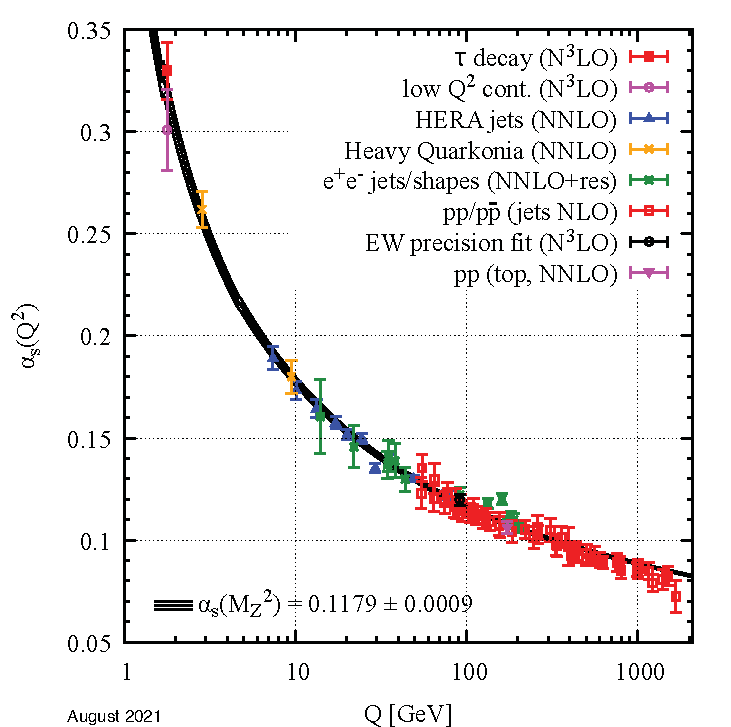
\includegraphics[width=\linewidth]{Assets/Plots/SM/QCD_alpha_s.pdf}
  \caption{Mediciones de la constante de acomplamiento de QCD, en función de la escala de energía. Se determina la constante $\alpha_s(M_Z^2)$ mediante un ajuste (en negro)~\citeonly{Zyla2020}.}
  \label{fig:ch1:SM:QCD:alpha_s}
\end{marginfigure}


\subsection{Interacción electrodébil}

La interacción electrodébil unifica las interacciones débiles y electromagnética, en un único grupo de simetría de gauge $SU(2)_L \times U(1)_Y$. Para garantizar la ruptura de simetría de paridad, observada experimentalmente en 1956 por Chien-Shiung Wu~\cite{Wu1957}, el SM expresa la interacción débil como una interacción de gauge quiral, solo produciendo cambios en los fermiones de quiralidad izquierda (dando orígen al subíndice $L$ en la definición del grupo $SU(2)_L$). Estos transforman como dobletes en la representación de definición de $SU(2)$ como
\[
  f_L \to U_{SU(2)_L} f_L = \exp\qty{i \frac{\sigma^i}{2} \theta^i} f_L,
  \quad \text{siendo} \quad
  f_L = \begin{pmatrix} \nu_L \\ e_L \end{pmatrix}, \begin{pmatrix} u_L \\ d_L \end{pmatrix}, \dots
\]
donde los generadores del grupo no abeliano se encuentran parametrizados por $T^i_{SU(2)_L} = \sigma^i/2$, siendo $\sigma^i$ las matrices de Pauli, mientras que los fermiones derechos lo hacen como singletes en la representación trivial ($T^i_{SU(2)_R} = 0$), con 
\[
  f_R \to U_{SU(2)_R} f_R = f_R,
  \quad \text{siendo} \quad
  f_R = e_R, u_R, d_R, \dots.
\]
Por el contrario, el grupo de hipercarga $U(1)_Y$ transforma en la representación de definición sobre todos los espinores, 
\[ f_{L/R} \to U_{U(1)_Y} f_{L/R} = \exp\qty{i g' \frac{Y}{2} \beta} f_{L/R}, \]
con un generador de simetría parametrizado como $T_{U(1)_Y} = y/2$.

Las cargas asociadas a los subgrupos de simetría $SU(2)_L$ y $U(1)_Y$ son conocidas como isospín débil ($t^a$, con $a = 1, 2, 3$), e hipercarga débil ($y$). Estas son compartidas entre las tres familias de quarks y leptones. Al encontrarse en la representación de definición, los fermiones izquierdos tienen un isospín débil total $t = 1/2$, siendo distinguidos en cada doblete por la proyección $t^3 = \pm 1/2$. Por el contrario, en la representación trivial, los fermiones de quiralidad derecha tendrán isospín débil $t = 0$. La hipercarga débil también resulta dependiente en la quiralidad, siendo determinada a partir de su relación con la carga eléctrica convencional $q$, dada por la misma fórmula que fue escrita por Gell-Mann y Nishijima para hadrones,
\begin{equation} q = t^3 + \frac{y}{2}. \label{eq:ch1:SM:Gell-Man_Nishijima} \end{equation}
Los números cuánticos electrodébiles de todos los fermiones del SM se encuentra en la \cref{tbl:ch1:SM:EW_isospin-charges}.

\begin{margintable}
  \centering
  \setlength{\tabcolsep}{1.5mm}
  \renewcommand{\arraystretch}{1.3}
  \begin{tabular}{clccc}
\toprule
                                                                                             &                                & $t^3$  & $y$    & $q$    \\
\midrule
\multirow{4}{*}{\rotatebox[origin=c]{90}{\parbox[c]{13mm}{\centering Quiralidad Izquierda}}} & $\nu_e$, $\nu_\mu$, $\nu_\tau$ & $+1/2$ & $-1$   & $0$    \\
                                                                                             & $e^-$, $\mu^-$, $\tau^-$       & $-1/2$ & $-1$   & $-1$   \\
                                                                                             & $u$, $c$, $t$                  & $+1/2$ & $+1/3$ & $+2/3$ \\
                                                                                             & $d$, $s$, $b$                  & $-1/2$ & $+1/3$ & $-1/3$ \\
\arrayrulecolor{black!50}\midrule\arrayrulecolor{black}
\multirow{3}{*}{\rotatebox[origin=c]{90}{\parbox[c]{13mm}{\centering Quiralidad Derecha}}}   & $e^-_R$, $\mu^-_R$, $\tau^-_R$ & $0$    & $-2$   & $-1$   \\
                                                                                             & $u_R$, $c_R$, $t_R$            & $0$    & $+4/3$ & $+2/3$ \\
                                                                                             & $d_R$, $s_R$, $b_R$            & $0$    & $-2/3$ & $-1/3$ \\
\bottomrule
\end{tabular}
  \caption{Isospín débil ($t^3$), hipercarga débil ($y$) y carga eléctrica ($Q$) de los fermiones presentes en el SM, de acuerdo a su quiralidad. No se incluyen neutrinos derechos, ya que (si existen) no interactuan por medio de la interacción electrodébil.}
  \label{tbl:ch1:SM:EW_isospin-charges}
\end{margintable}

El número de bosones de gauge asociados coincide con el número de generadores del groupo de simetría. Para el isospín débil se tienen 3 bosones de $SU(2)_L$, $W_\mu^i$, y para $U(1)_Y$ se tiene un bosón de hipercarga $B_\mu$. En analogía al tratamiento realizado para QCD, definimos tensores de campos de Gauge
\[
  W^i_{\mu\nu} = \partial_\mu W^i_\nu - \partial_\nu W^i_\mu + g \epsilon^{ijk} W^j_\mu W^k_\nu,
  \quad \text{y} \quad
  B_{\mu\nu} = \partial_\mu B_\nu - \partial_\nu B_\mu.
\]
La derivada covariante tomará en este caso una forma distinta para los dobletes de fermiones izquierdos y los singletes derechos, como
\begin{equation}
  D_\mu^L = \partial_\mu - i g \frac{\sigma^i}{2} W^i_\mu - i g' \frac{y}{2} B_\mu,
  \quad \text{y} \quad
  D_\mu^R = \partial_\mu - i g' \frac{y}{2} B_\mu.
  \label{eq:ch1:SM:EW_covariant_D}
\end{equation}
La densidad lagrangiana de la teoría resulta entonces
\[\Lag_{SM} \supset \Lag_{EW} = -\inv{4} W^{i\mu\nu} W^i_{\mu\nu} - \inv{4} B^\mu B_\mu + i \sum_{f = l, q} \qty[ \bar{f}_L \slashed{D}^L f_L + \bar{f}_R \slashed{D}^R f_R ]. \]
No es posible añadir términos de masa de Dirac explícitos al lagrangiano, ya que estos resultarían en la ruptura de la simetría electrodébil al mezclar los dobletes de quiralidad izquierda y los singletes de quiralidad derecha:
\[ -m_f \bar{f} f = -m(\bar{f}_L f_R + \bar{f}_R f_L). \]
Tampoco es posible añadir términos de masa para los mediadores electrodébiles ya que se rompería la simetría de Gauge, aunque experimentalmente se ha verificado que 3 de ellos son partículas muy masivas. El mecanismo por el cual estas partículas adquieren masa es conocido como Mecanismo de Higgs, y será tratado en la siguiente sección.







\subsection{Ruptura espontánea de la simetría electrodébil}

El mecanismo de Higgs\sidenote[][-8em]{Si bien suele solo llevar el nombre de Peter Higgs, este mecanismo fue descubierto de manera independiente y simultánea por tres grupos en 1964: por Robert Brout y François Englert~\cite{Englert1964}; por Peter Higgs~\cite{Higgs1964}; y por Gerald Guralnik, Carl R. Hagen y Thomas Kibble~\cite{Guralnik1964}.}~\cite{Higgs1964} implica el rompimiento espontáneo de la simetría electrodébil $SU(2)_L \times U(1)_Y$ en $U(1)_{EM}$, asociado al electromagnetismo y provee las masas de los fermiones y 3 de los 4 bosones electrodébiles observados experimentalmente\sidenote[][-1.2em]{Por el Teorema de Goldstone, sabemos que la ruptura de 3 simetrías contínuas de la teoría resultará en 3 bosones de Goldstone (no masivos), que son \textit{absorbidos} mediante transformaciones locales de gauge por 3 campos de gauge, adquiriendo masa.}, $W^\pm$ y $Z^0$ (combinaciones lineales de los campos $W^i_\mu$ y $B_\mu$). Para ello, se introduce un nuevo campo escalar complejo $\Phi$, llamado \textit{campo de Higgs}, en la representación de definición de $SU(2)$
\[ \Phi = \begin{pmatrix} \phi_+ \\ \phi_0 \end{pmatrix}, \]
donde $\phi_+$ y $\phi_0$ poseen la carga eléctrica indicada por sus subíndices, por lo que $y_\Phi = 1$. La dinámica de este campo escalar es añadida al SM como
\[ \Lag_{SM} \supset \Lag_{H} = (D^\mu \Phi)^\dagger D_\mu \Phi - V(\abs{\Phi}), \]
acoplando con los bosones $W^i_\mu$ y $B_\mu$ por medio de la derivada covariante $D_\mu = D^L_\mu$ definida en \eqref{eq:ch1:SM:EW_covariant_D}. Para obtener un valor de expectación de vacío (vev) del campo no nulo y romper espontáneamente la simetría electrodébil, introducimos el potencial de Higgs
\[ V(\abs{\Phi}) = \mu^2 \Phi^\dagger \Phi + \lambda (\Phi^\dagger \Phi)^2, \]
invariante ante transformaciones locales de $SU(2)_L$. Para acotar su magnitud mínima, se requiere $\lambda > 0$. Si $\mu^2 > 0$, el potencial tendrá un único mínimo en $\abs{\Phi} = 0$. Sin embargo, si $\mu^2 < 0$, el potencial toma la forma de \textit{sombrero mexicano} (\cref{fig:ch1:SM:Higgs_potential}), con un estado fundamental infinitamente degenerado en $\abs{\Phi} = v/\sqrt{2}$, donde $v = \sqrt{-\mu^2/\lambda} \approx \SI{246.22}{\GeV}$ es el vev del campo de Higgs, usualmente elegido como
\[ \mel{0}{\Phi}{0} = \begin{pmatrix} 0 \\ \frac{v}{\sqrt{2}} \end{pmatrix}. \]

Sin pérdida de generalidad, podemos reparametrizar el campo de Higgs alrededor del vev, rotando sus componentes mediante una transformación local de componentes $\theta^i(x)$ a
\[ \Phi = \exp\qty{i \frac{\sigma^i}{2} \theta^i} \begin{pmatrix} 0 \\ \frac{v}{\sqrt{2}} + \frac{h}{\sqrt{2}} \end{pmatrix}. \]
Los tres campos $\theta^i(x)$ serían identificados como bosones de Goldstone, asociados a los grados de libertad no radiales del campo, que son eliminados mediante una transformación del gauge local $SU(2)_L$. Al eliminarse, los 3 grados de libertad de los modos de Goldstone son \textit{absorbidos} por 3 bosones de gauge de la teoría electrodébil, dándoles masa.

\begin{marginfigure}[-20em]
  \centering
  \resizebox{0.99\linewidth}{!}{
\begin{tikzpicture}
    \begin{axis}[
            axis y line = center,
            axis x line = middle,
            axis line style = {-{Latex[scale=2]}, very thin, darkgray},
            ticks = none,
            clip = false,
            xmin = -2.2, xmax = 2.2,
            ymin = -3, ymax = 15,
        ]
        \addplot[domain=-2:2, smooth, samples=100, thick] {-5*x^2 + 2*x^4};
        %
        \node at (axis cs:0.5, 15) {\large$V(\abs{\Phi})$};
        \node at (axis cs:2, -1.5) {\large$\Re(\Phi)$};
        \draw[-{Latex[scale=2]}, very thin] (axis cs:0, 0) -- (axis cs:-1.5, -6);
        \node at (axis cs:-0.8, -6) {\large$\Im(\Phi)$};
        %
        \coordinate (el_0_c) at (axis cs:0, -3.125);
        \coordinate (el_0_e) at (axis cs:1.11801, -3.125);
        \coordinate (el_1_c) at (axis cs:0, 4);
        \coordinate (el_1_e) at (axis cs:1.77129, 4);
        \coordinate (el_2_c) at (axis cs:0, 9);
        \coordinate (el_2_e) at (axis cs:1.92671, 9);
        %
        \coordinate (el_0_e_axis) at (axis cs:1.11801, 0);
    \end{axis}
    \newlength{\rx}
    \pgfextractx{\rx}{\pgfpointdiff{\pgfpointanchor{el_0_e}{center}}{\pgfpointanchor{el_0_c}{center}}}%
    \draw[dashed, darkgray] (el_0_c) ellipse [x radius = \rx, y radius = 3mm];
    \pgfextractx{\rx}{\pgfpointdiff{\pgfpointanchor{el_1_e}{center}}{\pgfpointanchor{el_1_c}{center}}}%
    \draw[dashed, darkgray] (el_1_c) ellipse [x radius = \rx, y radius = 3mm];
    \pgfextractx{\rx}{\pgfpointdiff{\pgfpointanchor{el_2_e}{center}}{\pgfpointanchor{el_2_c}{center}}}%
    \draw[dashed, darkgray] (el_2_c) ellipse [x radius = \rx, y radius = 3mm];
    %
    \draw[dashed, darkgray] (el_0_e) -- (el_0_e_axis);
    \node[circle, fill=Burgundy, inner sep=1mm] at (el_0_e) {};
    \node at ([shift={(-1mm, 4.5mm)}] el_0_e_axis) {\normalsize$v = \sqrt{-\frac{\mu^2}{\lambda}}$};
\end{tikzpicture}
}
  \caption{Potencial de Higgs $V(\abs{\Phi})$, para $-\mu^2 < 0$.}
  \label{fig:ch1:SM:Higgs_potential}
\end{marginfigure}

A bajas energías, las resonancias de mediadores electrodébiles que se observan experimentalmente no son excitaciones de los campos $W^i_\mu$ y $B_\mu$, sino combinaciones de ellos, que se corresponden con los términos diagonales y no-diagonales de la matríz de gauge asociada a la derivada covariante:
\[
  D_\mu \Phi = \partial_\mu + i \frac{g}{\sqrt{2}}
  \begin{pmatrix}
    \inv{g\sqrt{2}}\qty(g W^3_\mu + g' B_\mu) & \inv{\sqrt{2}} \qty(W^1_\mu - i W^2_\mu)  \\
    \inv{\sqrt{2}} \qty(W^1_\mu + i W^2_\mu)  & \inv{g\sqrt{2}}\qty(g' W^3_\mu - g B_\mu)
  \end{pmatrix}.
\]
Bajo la normalización usual,
\[ 
  W^\pm_\mu = \inv{\sqrt{2}}(W^1_\mu \mp i W^2_\mu), 
  \quad 
  Z^0_\mu = \frac{g W^3_\mu - g' B_\mu}{\sqrt{g^2+g'^2}},
  \quad
  A_\mu = \frac{g' W^3_\mu + g B_\mu}{\sqrt{g^2+g'^2}},
\]
por lo que al desarrollar el término cinético del campo de Higgs, a orden $\mathcal{O}(h^0)$, obtenemos los términos de masa efectiva
\[ \Lag_{H} \supset \Lag_{W^\pm, Z^0 \text{mass}} = m_W^2 W^+_\mu W^{-\mu} + \inv{2} m_Z^2 Z_\mu Z^\mu, \]
con
\[ m_W = \frac{gv}{2} = \frac{m_H^2 g}{4\lambda}, \quad m_Z = \frac{v}{2}\sqrt{g^2 + g'^2} = \frac{m_H^2}{4\lambda} \sqrt{g^2 + g'^2}. \]
El campo de $A_\mu$ permanece sin masa, correspondiéndose a la simetría de Gauge resultante $U(1)_{EM}$. La masa del campo de Higgs, $m_H = \sqrt{-2\mu^2}$, es obtenida desarrollando el potencial de Higgs a órden $\mathcal{O}(h^2)$.

Los vértices de interacción resultantes entre bosones electrodébiles y fermiones se encuentran descritos en la \cref{fig:ch1:SM:EW:vertices}. Para mediar las transformaciones entre fermiones de isospín semientero de distinta proyección $t^3$, los bosones de gauge deberán tener isospín total $t = 1$. Los bosones $W^\pm$, con $t^3_{W^\pm} = \pm 1$, se emiten en las transiciones $t^3 = \pm 1/2 \to t^3 = \mp 1/2$. Por el contrario, en transiciones neutras $t^3 = \pm 1/2 \to t^3 = \pm 1/2$, como en el scattering electromagnético o de neutrinos, se da la emisión de bosones $Z^0$ y $A$, ambos con isospín débil $t^3_{Z,A} = 0$. Las interacciones electromagnéticas dependerán de la carga eléctrica $q$, obtenida en \eqref{eq:ch1:SM:Gell-Man_Nishijima}, mientras que las interacciones mediadas por bosones $Z^0$ tendrán una carga débil asociada 
\[ q_z = \frac{t^3 - q \sin^2\theta_w}{\sin\theta_w \cos\theta_w}, \]
donde $\tan\theta_w = g'/g$, soendo $\theta_w$ el ángulo de Weinberg.

\begin{marginfigure}
  \centering
  \begin{align*}
    &\feynmandiagram [small, inline=(vert.base), horizontal=i to vert] {
      i [particle=\( W^\pm\)] -- [photon] vert,
      f1 [particle=\( \text{$\nu^e$, $\nu^\mu$, $\nu^\tau$} \)] -- [anti fermion] vert -- [anti fermion] f2 [particle=\( \text{$\bar{e}$, $\bar{\mu}$, $\bar{\tau}$} \)],
    };
    \hspace{-8pt}
    \propto \frac{g}{2\sqrt{2}} (1 - \gamma_5),\\
    %
    &\feynmandiagram [small, inline=(vert.base), horizontal=i to vert] {
      i [particle=\(W^\pm\)] -- [photon] vert,
      f1 [particle=\( \text{$u$, $c$, $t$} \)] -- [anti fermion] vert -- [anti fermion] f2 [particle=\( \text{$\bar{d}$, $\bar{s}$, $\bar{b}$} \)],
    };
    \propto \frac{g}{2\sqrt{2}} (1 - \gamma_5) V_{ud},\\
    %
    &\feynmandiagram [small, inline=(vert.base), horizontal=i to vert] {
      i [particle=\(\gamma\)] -- [photon] vert,
      f1 [particle=\( \text{$q$, $l$} \)] -- [anti fermion] vert -- [anti fermion] f2 [particle=\( \text{$\bar{q}$, $\bar{l}$} \)],
    };
    \hspace{7pt}
    \propto e q,\\
    %
    &\feynmandiagram [small, inline=(vert.base), horizontal=i to vert] {
      i [particle=\(Z^0\)] -- [photon] vert,
      f1 [particle=\( \text{$q$, $l$, $\nu_L$} \)] -- [anti fermion] vert -- [anti fermion] f2 [particle=\( \text{$\bar{q}$, $\bar{l}$, $\bar{\nu}_L$} \)],
    };
    \hspace{0.5pt}
    \propto e q_z.
  \end{align*}
  \caption{Vértices de interacciones electrodébiles. En las interacciones cargadas entre quarks y los mediadores cargados $W^\pm$, $V_{ud}$ es el elemento de la matríz CKM de los quarks tipo-$u$ y tipo-$d$ del vértice.}
  \label{fig:ch1:SM:EW:vertices}
\end{marginfigure}

El mecanismo de Higgs también es responsable de asignar masas a los fermiones del SM, incluyendo en el lagrangiano acoplamientos de Yukawa de la forma:
\begin{align*}
  \Lag_{SM} \supset \Lag_{Y} &= -\sum_{i = 1}^3 Y^e_{i} \ \bar{l}_L^i \Phi e_R^i -\sum_{i,j =1}^3 \qty[ Y_{ij}^d \ \bar{q}_L^i \Phi d^j_R + Y_{ij}^u \ \bar{q}_L^i \tilde{\Phi} u^j_R ] + \text{h.c.} \\
    &= -\sum_{i = 1}^3 \frac{v}{\sqrt{2}} Y^e_{i} (\bar{e}_L^i e_R^i + \bar{e}_R^i e_L^i) \\
    &\quad - \sum_{i,j =1}^3 \frac{v}{\sqrt{2}} \qty[ Y_{ij}^d \ \bar{q}_L^i \Phi d^j_R + Y_{ij}^u \ \bar{q}_L^i \tilde{\Phi} u^j_R ] + \mathcal{O}(h^1) + \text{h.c.},
\end{align*}
donde $i$ y $j$ son los índices de la generación de los fermiones (tal que $u^i_R = (u_R, c_R, t_R)$ y lo mismo para los quarks tipo-$d$ y los leptones) y $\tilde{\Phi} = i \sigma^2 \Phi$. Los términos de masa de Dirac de los leptones cargados se hacen explícitos con solo desarrollar $\Lag_Y$ a orden $\mathcal{O}(h^0)$, resultando en $m_{e^i} = v Y^e_i / \sqrt{2}$. Sin embargo, en el caso de los quarks, las matrices de Yukawa $Y^u_{ij}$ e $Y^d_{ij}$ requieren una diagonalización
\[ Y^u = U^u M^u {K^u}^\dagger \quad \text{y} \quad Y^d = U^d M^d {K^d}^\dagger \]
para obtener los autoestados de masa, ahora con $m_{u^i} = v M^u_{ii} /\sqrt{2}$ y una expresión análoga para $m_{d^i}$. La matríz $V = {U^u}^\dagger U^d$, conocida como matríz CKM (Cabibbo-Kobayashi-Maskawa), contiene toda la información de la mezcla de los autoestados de sabor de los quarks que ocurre en la interacción débil cargada. Al contener una fase no nula ($V^* \neq V$), la matriz CKM da origen a la violación de la simetría $CP$ (conjugación de carga-paridad) en el SM.

Los neutrinos son los únicos fermiones que no adquirirían masa por el mecanismo de Higgs, al no incorporarse en el SM un término de Yukawa que relacione sus campos con el campo de Higgs.










\subsection{Interacciones hadrónicas en un colisionador protón-protón} \label{sec:ch1:SM:had_interactions}

\begin{marginfigure}
  \centering
  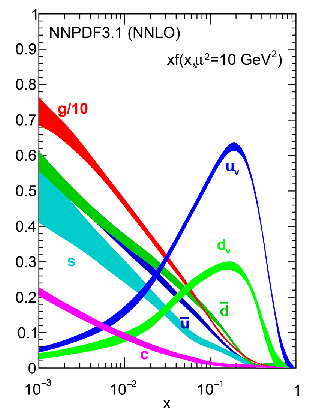
\includegraphics[width=0.99\marginparwidth]{Assets/Plots/SM/NNPDF_PDF_mu2-10GeV2.pdf}\\
  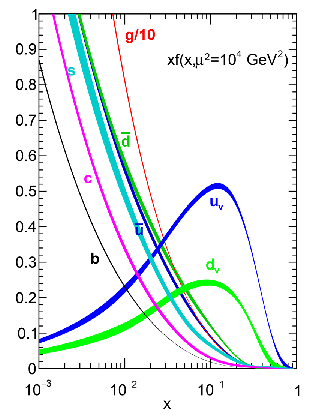
\includegraphics[width=0.99\marginparwidth]{Assets/Plots/SM/NNPDF_PDF_mu2-10000GeV2.pdf}
  \caption{Funciones de distribución partónica (PDF) usando predicciones NNLO (\textit{next-to-next-to-leading order}) de quarks y gluones en protones, para escalas de factorización $\mu_F^2$ \SI{10}{\GeV^2} y $10^4\si{\GeV^2}$~\citeonly{DelDebbio2018}.}
  \label{fig:ch1:SM:pp_interactions:pdf}
\end{marginfigure}

Como se ha discutido en la \cref{sec:ch1:SM:QCD}, la constante de acoplamiento $\alpha_s$, que gobierna las interacciones fuertes entre quarks, tiene una fuerte dependencia en la escala de energía de cada interacción, modificando radicalmente la naturaleza de los procesos. El modelado de una colisión protón-protón en un experimento como ATLAS, donde se requiere conocer su evolución desde la interacción entre los protones a $\sqrt{s} = \SI{13}{\TeV}$, hasta la interacción de las partículas en el estado final con los materiales activos y pasivos del detector a unos pocos \si{\GeV}, representa un enorme desafío, al cubrir regímenes de QCD con comportamientos muy distintos en sus extremos.

A altas energías (más precisamente, a altas transferencias de impulso), en el régimen perturbativo, la colisión entre dos protones puede ser estudiada por medio del modelo de partones, tratando a los hadrones como objetos compuestos de partículas puntuales con interacciones de muy corta distancia. Este modelo fue introducido por Richard Feynman en 1969 y aplicado inmediatamente por Bjorken y Paschos para interpretar los resultados de los experimentos de dispersión inelástica profunda electrón-nucleón en SLAC. Bajo esta abstracción, los partones no solo incluyen a los quarks de valencia ($u$, $u$ y $d$ en el caso del protón), sino también los pares de partículas y antipartículas del mar de quarks, y los gluones que median las interacciones entre ellos. El modelo supone una permanente interacción entre partones, por lo que su momento individual resulta desconocido, aunque su fracción de momento respecto al momento total del hadrón puede ser modelado como una variable aleatoria.

A bajas energías, como ya hemos mencionado en \ref{sec:ch1:SM:QCD}, el principio de confinamiento obliga a los quarks y gluones libres a \textit{hadronizar}, formando nuevamente estados ligados sin color mediante la producción de pares quarks-antiquarks. Este proceso resulta en la formación de jets hadrónicos, modelados fenomenológicamente, que pueden ser observados en el detector, como será desarrollado en los \cref{chap:ch2,chap:ch3}.

\begin{marginfigure}
  \centering
  \begin{tikzpicture}
    \coordinate (a1_i) at (0mm,0mm);
    \coordinate[below=2mm of a1_i] (a2_i);
    \coordinate[below=2mm of a2_i] (a3_i);
    %
    \coordinate[right=22mm of a1_i] (a1_m);
    \coordinate[right=22mm of a2_i] (a2_m);
    \coordinate[right=22mm of a3_i] (a3_m);
    %
    \coordinate[above right=7mm and 20mm of a1_m] (a1_e);
    \coordinate[above right=7mm and 20mm of a2_m] (a2_e);
    %
    \coordinate[below=14mm of a3_i] (b1_i);
    \coordinate[below=2mm of b1_i] (b2_i);
    \coordinate[below=2mm of b2_i] (b3_i);
    %
    \coordinate[right=22mm of b1_i] (b1_m);
    \coordinate[right=22mm of b2_i] (b2_m);
    \coordinate[right=22mm of b3_i] (b3_m);
    %
    \coordinate[below right=7mm and 20mm of b2_m] (b2_e);
    \coordinate[below right=7mm and 20mm of b3_m] (b3_e);
    %
    \coordinate[below right=7mm and 10mm of a3_m] (middle);
    %
    \begin{scope}[thick, decoration={markings, mark=at position 0.4 with {\arrow{latex}}}]
        \draw[postaction={decorate}] (a1_i) -- (a1_m);
        \draw[postaction={decorate}] (a2_i) -- (a2_m);
        \draw[postaction={decorate}] (a3_i) -- (a3_m);
        %
        \draw[postaction={decorate}] (b1_i) -- (b1_m);
        \draw[postaction={decorate}] (b2_i) -- (b2_m);
        \draw[postaction={decorate}] (b3_i) -- (b3_m);
    \end{scope}
    %
    \begin{scope}[thick, decoration={markings, mark=at position 0.6 with {\arrow{latex}}}]
        \draw[postaction={decorate}] (a1_m) -- (a1_e);
        \draw[postaction={decorate}] (a2_m) -- (a2_e);
        %
        \draw[postaction={decorate}] (b2_m) -- (b2_e);
        \draw[postaction={decorate}] (b3_m) -- (b3_e);
    \end{scope}
    %
    \begin{scope}[thick, decoration={markings, mark=at position 0.8 with {\arrow{latex}}}]
        \draw[postaction={decorate}] (a3_m) -- (middle);
        \draw[postaction={decorate}] (b1_m) -- (middle);
    \end{scope}
    %
    \node at ([shift={(2mm, 3mm)}]a1_i) {\large$A$};
    \node at ([shift={(2mm, -3mm)}]b3_i) {\large$B$};
    %
    \coordinate[left=2mm of a2_m] (a_circle);
    \filldraw[color=Burgundy, fill=white, thick] (a_circle) circle (7mm);
    \node at (a_circle) {\large$f_{A/a_i}$};
    \coordinate[left=2mm of b2_m] (b_circle);
    \filldraw[color=Burgundy, fill=white, thick] (b_circle) circle (7mm);
    \node at (b_circle) {\large$f_{B/b_i}$};
    %
    \node at ($(a3_m)!0.8!(middle) + (-0.5mm, 3mm)$) {$x_{a_i}$};
    \node at ($(b1_m)!0.8!(middle) + (-0.5mm, -4mm)$) {$x_{b_j}$};
    %
    \node[draw, fit={([shift={(1mm, 2mm)}] middle) ([shift={(15mm, -2mm)}] middle)}, preaction={fill=white}, color=Burgundy, label={[align=center]center:\large$\hat{\sigma}_{a_i b_j \to X}$}] (sigma) {};
    %
    \draw [-{Implies[]}, double distance=0.6mm, thick] (sigma.east) -- ([shift={(8mm, 0mm)}] sigma.east);
    \node at ([shift={(5.5mm, 4mm)}] sigma.east) {\large$X$};
\end{tikzpicture}
  \caption{Ilustración esquemática del proceso de factorización en una colisión pp, donde un partón de cada protón sufre una dispersión dura.}
  \label{fig:ch1:SM:pp_interactions:factorization}
\end{marginfigure}

La conexión entre estos dos regímenes es posible gracias al concepto de \textit{factorización}, ideado por Feynman~\cite{Feynman1969}, que permite una separación sistemática entre las interacciones de corta distancia (entre partones) y las interacciones de larga distancia (entre hadrones). El teorema de factorización~\cite{Collins1989}, ilustrado esquemáticamente en la \cref{fig:ch1:SM:pp_interactions:factorization} para una interacción entre dos bariones, establece que la sección eficaz de producción de cualquier proceso de QCD del tipo $A + B \to X$ puede ser estimada como
\begin{equation}
  \sigma_{AB \to X} = \sum_{ij} \int \dd{x_{a_i}} \dd{x_{b_j}} f_{A/a_i}(x_{a_i}, \mu_F^2) f_{B/b_j}(x_{b_j}, \mu_F^2) \hat{\sigma}_{a_i b_j \to X}(\mu_F^2, \mu_R^2), \label{eq:ch1:SM:factorization}
\end{equation}
donde $x_i$ y $x_j$ son las fracciones del momento de los hadrones $A$ y $B$, que llevan los partones $a_i$ y $b_j$ respectivamente, y $\hat{\sigma}_{a_i b_j}$ es la sección eficaz de la interacción a nivel partónico, calculada a un dado orden de perturbaciones y una escala de renormalización $\mu_R$. Esta escala de normalización es importante para absorber las divergencias UV en los cálculos a órdenes mayores. Las funciones $f_{H/p}(x_p,\mu_F^2)$ son las funciones de distribución partónicas, o PDFs, que representan la probabilidad de encontrar un partón de tipo $p$ en un hadrón $H$ con una fracción de momento $x_p$, dada la escala de factorización $\SI{1}{\GeV^2} \leq \mu_F \leq Q^2$. Esta escala se introduce para tratar singularidades que aparecen en el regimen no perturbativo. Las PDFs no pueden ser determinadas perturbativamente, pero su dependencia funcional con la escala de energía se puede predecir con las ecuaciones DGLAP (Dokshitzer-Gribov-Lipatov-Altarelli-Parisi)~\citeonly{Gribov1971,Altarelli1977,Dokshitzer1977}. Para el caso del protón, las PDFs son exhibidas en la \cref{fig:ch1:SM:pp_interactions:pdf}.

\begin{marginfigure}[2em]
  \centering
  \begin{tikzpicture}
    \begin{feynman}
        \vertex (i) {\(q\)};
        \vertex[below=15mm of i] (l1v1);
        \vertex[below left=10mm and 12mm of l1v1] (l2v1);
        \vertex[below right=10mm and 12mm of l1v1] (l2v2);
        \vertex[below left=10mm and 6mm of l2v1] (l3v1);
        \vertex[below right=10mm and 6mm of l2v1] (l3v2);
        \vertex[below left=10mm and 6mm of l2v2] (l3v3);
        \vertex[below right=10mm and 6mm of l2v2] (l3v4);
        \vertex[below left=10mm and 6mm of l3v2] (l4v1);
        \vertex[below right=10mm and 6mm of l3v2] (l4v2);
        \vertex[below left=10mm and 6mm of l3v4] (l4v3);
        \vertex[below right=10mm and 6mm of l3v4] (l4v4);
        \vertex[below=17mm of l3v1] (l5v1);
        \vertex[below=7mm of l4v1] (l5v2);
        \vertex[below=7mm of l4v2] (l5v3);
        \vertex[below=17mm of l3v3] (l5v4);
        \vertex[below=7mm of l4v3] (l5v5);
        \vertex[below=7mm of l4v4] (l5v6);
        %
        \diagram*{
        (i) -- [fermion] (l1v1),
        (l2v1) -- [gluon, edge label=\(g\)] (l1v1) -- [fermion, edge label=\(q\)] (l2v2),
        (l3v1) -- [fermion, edge label=\(\bar{q}\)] (l2v1) -- [fermion, edge label=\(q\)] (l3v2),
        (l3v3) -- [anti fermion, edge label=\(q\)] (l2v2) -- [gluon, edge label=\(g\)] (l3v4),
        (l4v1) -- [anti fermion, edge label=\(q\)] (l3v2) -- [gluon, edge label=\(g\)] (l4v2),
        (l4v3) -- [fermion, edge label=\(\bar{q}\)] (l3v4) -- [fermion, edge label=\(q\)] (l4v4),
        (l3v1) -- [ghost] (l5v1),
        (l4v1) -- [ghost] (l5v2),
        (l4v2) -- [ghost] (l5v3),
        (l3v3) -- [ghost] (l5v4),
        (l4v3) -- [ghost] (l5v5),
        (l4v4) -- [ghost] (l5v6),
        };
    \end{feynman}
    %
    \node[fit={([shift={(-3mm, 0mm)}] l5v1) ([shift={(3mm, -10mm)}] l5v6)}, preaction={fill=white}, pattern=north west lines, pattern color=lightgray, label={[text=darkgray]center:\small\smallcaps{Hadronización}}] (hadronization) {};
    \draw [color=Burgundy] (hadronization.north west) -- (hadronization.north east) (hadronization.south west) -- (hadronization.south east);
    %
    \begin{feynman}
        \vertex[above right=0mm and 6mm of hadronization.south west] (h1l1v1);
        \vertex[below right=12mm and -1mm of h1l1v1] (h1l2v1);
        \vertex[below right=18mm and -3mm of h1l2v1] (h1l5v1);
        \vertex[below right=18mm and -2mm of h1l2v1] (h1l5v2);
        \vertex[below right=18mm and -1mm of h1l2v1] (h1l5v3);
        \vertex[below right=18mm and 1mm of h1l2v1] (h1l5v4);
        \vertex[below right=18mm and 2mm of h1l2v1] (h1l5v5);
        \vertex[below right=18mm and 3mm of h1l2v1] (h1l5v6);
        \vertex[below right=18mm and 9mm of h1l2v1] (h1l5v7);
        \vertex[below right=6mm and -2mm of h1l2v1] (h1l3v1);
        \vertex (h1l3v2) at ($(h1l2v1)!0.4!(h1l5v5)$);
        \vertex (h1l3v3) at ($(h1l2v1)!0.5!(h1l5v7)$);
        \vertex (h1l4v1) at ($(h1l2v1)!0.55!(h1l5v5)$);
        %
        \vertex[above right=0mm and 14mm of hadronization.south west] (h2l1v1);
        \vertex[below right=30mm and -3mm of h2l1v1] (h2l3v1);
        \vertex[below right=30mm and 4mm of h2l1v1] (h2l3v2);
        \vertex (h2l2v1) at ($(h2l1v1)!0.35!(h2l3v1)$);
        %
        \vertex[above right=0mm and 21mm of hadronization.south west] (h3l1v1);
        \vertex[below right=6mm and -1mm of h3l1v1] (h3l2v1);
        \vertex[below right=24mm and -4mm of h3l2v1] (h3l3v1);
        \vertex[below right=24mm and 4mm of h3l2v1] (h3l3v2);
        %
        \vertex[above right=0mm and 26mm of hadronization.south west] (h4l1v1);
        \vertex[below right=24mm and -1mm of h4l1v1] (h4l2v1);
        \vertex[below right=6mm and -2mm of h4l2v1] (h4l3v1);
        \vertex[below right=6mm and 4mm of h4l2v1] (h4l3v2);
        %
        \vertex[above right=0mm and 30mm of hadronization.south west] (h5l1v1);
        \vertex[below right=30mm and 1mm of h5l1v1] (h5l2v1);
        %
        \vertex[above right=0mm and 38mm of hadronization.south west] (h6l1v1);
        \vertex[below right=30mm and -2mm of h6l1v1] (h6l2v1);
        %
        \vertex[above right=0mm and 40mm of hadronization.south west] (h7l1v1);
        \vertex[below right=30mm and -1mm of h7l1v1] (h7l2v1);
        %
        \vertex[above right=0mm and 44mm of hadronization.south west] (h8l1v1);
        \vertex[below right=20mm and 1mm of h8l1v1] (h8l2v1);
        \vertex[below right=10mm and -4mm of h8l2v1] (h8l4v1);
        \vertex (h8l3v1) at ($(h8l2v1)!0.4!(h8l4v1)$);
        \vertex[below right=10mm and -2mm of h8l2v1] (h8l4v2);
        \vertex[below right=10mm and -1mm of h8l2v1] (h8l4v3);
        \vertex[below right=10mm and 2mm of h8l2v1] (h8l4v4);
        %
        \diagram*{
        (h1l1v1) -- (h1l2v1);
        (h1l2v1) -- (h1l3v1);
        (h1l3v1) -- (h1l5v1);
        (h1l3v2) -- (h1l5v2);
        (h1l4v1) -- (h1l5v3);
        (h1l3v1) -- (h1l5v4);
        (h1l2v1) -- (h1l5v5);
        (h1l3v3) -- (h1l5v6);
        (h1l2v1) -- (h1l5v7);
        %
        (h2l1v1) -- (h2l3v1);
        (h2l2v1) -- (h2l3v2);
        %
        (h3l1v1) -- (h3l2v1);
        (h3l2v1) -- (h3l3v1);
        (h3l2v1) -- (h3l3v2);
        %
        (h4l1v1) -- (h4l2v1);
        (h4l2v1) -- (h4l3v1);
        (h4l2v1) -- (h4l3v2);
        %
        (h5l1v1) -- (h5l2v1);
        %
        (h6l1v1) -- (h6l2v1);
        %
        (h7l1v1) -- (h7l2v1);
        %
        (h8l1v1) -- (h8l2v1);
        (h8l2v1) -- (h8l4v1);
        (h8l3v1) -- (h8l4v2);
        (h8l2v1) -- (h8l4v3);
        (h8l2v1) -- (h8l4v4);
        };
    \end{feynman}
    %
    \node[fit={([shift={(0mm, -36mm)}] hadronization.south west) ([shift={(0mm, -38mm)}] hadronization.south east)}, align=center] (exp_hadrons) {\small\(\pi^\pm, \pi^0, K^\pm, K^0, \dots\)};
    %
    \node[fit={([shift={(-5mm, -1mm)}] hadronization.north west |- l1v1) ([shift={(-2mm, 2mm)}] hadronization.north west)}, label={[label distance=5mm, rotate=90, text=darkgray]center:\smallcaps{Lluvia partónica}}] (parton_shower) {};
    \draw[dashed, color=Burgundy] (parton_shower.north east) -- (parton_shower.south east);
    %
    \node[fit={([shift={(-5mm, -2mm)}] hadronization.south west) ([shift={(-2mm, 0mm)}] hadronization.west |- exp_hadrons.south west)}, label={[label distance=5mm, rotate=90, text=darkgray]center:\smallcaps{Decaimiento de hadrones}}] (hadron_decay) {};
    \draw[dashed, color=Burgundy] (hadron_decay.north east) -- (hadron_decay.south east);
\end{tikzpicture}
  \caption{Diagrama del proceso de una lluvia partónica, hadronización y decaimiento de hadrones inestables a hadrones estables, comenzando con un quark $q$ producido en la interacción.}
  \label{fig:ch1:SM:pp_interactions:hadron_production}
\end{marginfigure}

El modelado de una colisión $pp$ comienza en el cálculo del elemento de matríz $M = \mel{f}{S}{i}$ de un proceso de dispersión dura (HS, \textit{Hard Scatter}) entre partones iniciales en el régimen perturbativo. Al igual que en el estudio de secciones eficaces de interacción en QFT tradicional, este contiene toda la información de las funciones de onda entrantes y salientes y depende de la escala de energía de dispersión.

Los partones pueden emitir quarks o gluones antes y después del proceso de HS, conocidos como radiación de estado inicial y final (ISR, \textit{initial state radiation}, y FSR, \textit{final state radiation}). Los partones que no participaron de la dispersión dura también pueden interactuar, dando lugar a interacciones de bajo momento (\textit{soft}), que conforman el \textit{evento subyacente} (UE, \textit{underlying event}). Al contener en su mayoría interacciones de menor energía, este requiere de tratamientos fenomenológicos no perturbativos.

Luego de la interacción principal de HS, todos los partones producidos en el estado final evolucionan radiando gluones \textit{soft} y quarks livianos, en un proceso conocido como \textit{lluvia} o \textit{cascada de partones} (PS, \textit{parton shower}). En cada paso de las cascadas partónicas, la probabilidad de fragmentación a un hadrón adicional $C$ se introduce a la eq. \eqref{eq:ch1:SM:factorization}
\[ \hat{\sigma}_{a_i b_j \to C + X} =  \sum_k \int \dd{z_C} D_{c_k}(z_C,\mu_f^2) \ \sigma_{a_i b_j \to c_k + X}(\mu_F^2, \mu_R^2), \]
donde $c_k$ es un partón con una probabilidad de fragmentar a $C$ determinada por la función de fragmentación $D_{c_k}(z_C, \mu_f)$, con una fracción $z_C$ de su momento, a la escala de fragmentación $\mu_f$. Este proceso finaliza al alcanzar la escala de hadronización $Q \sim \SI{1}{\GeV}$, donde el tratamiento de QCD deja de ser perturbativo y los partones en el estado final de la cascada son recombinados en hadrones por el principio de confinamiento. Esta fase es explicada por algunos modelos fenomenológicos~\cite{Bahr2008}. 

Algunos hadrones producidos en la etapa de hadronización son muy inestables, con vidas medias muy pequeñas, no alcanzando a ser observados directamente. Estos hadrones decaerán rápidamente en otros hadrones más estables, como piones y kaones, que serán observados por el detector. Nuevamente, en esta etapa final no podemos recurrir a QCD ya que nos encontramos en régimenes de baja energía (bajas transferencias de impulsos), por lo que se emplean modelos fenomenológicos, utilizando \textit{branching ratios}\sidenote[][-2em]{Se define el \textit{branching ratio} (o \textit{branching fraction}) como la fracción de partículas que decaen mediante un canal particular, respecto al número total de partículas que decaen.} determinados experimentalmente para los distintos hadrones.

Este proceso de múltiples etapas se encuentra representado esquemáticamente en la \cref{fig:ch1:SM:pp_interactions:hadron_production}, para el caso de un quark inicial.

Los cálculos teóricos de las secciones eficaces de los procesos del Modelo Estándar producidos en los colisionadores hadrónicos presentan un muy buen acuerdo con las mediciones experimentales, como podemos observar en la \cref{fig:ch1:SM:pp_interactions:cross_sections}~\cite{ATL-PHYS-PUB-2021-032}.

\begin{figure}[t]
  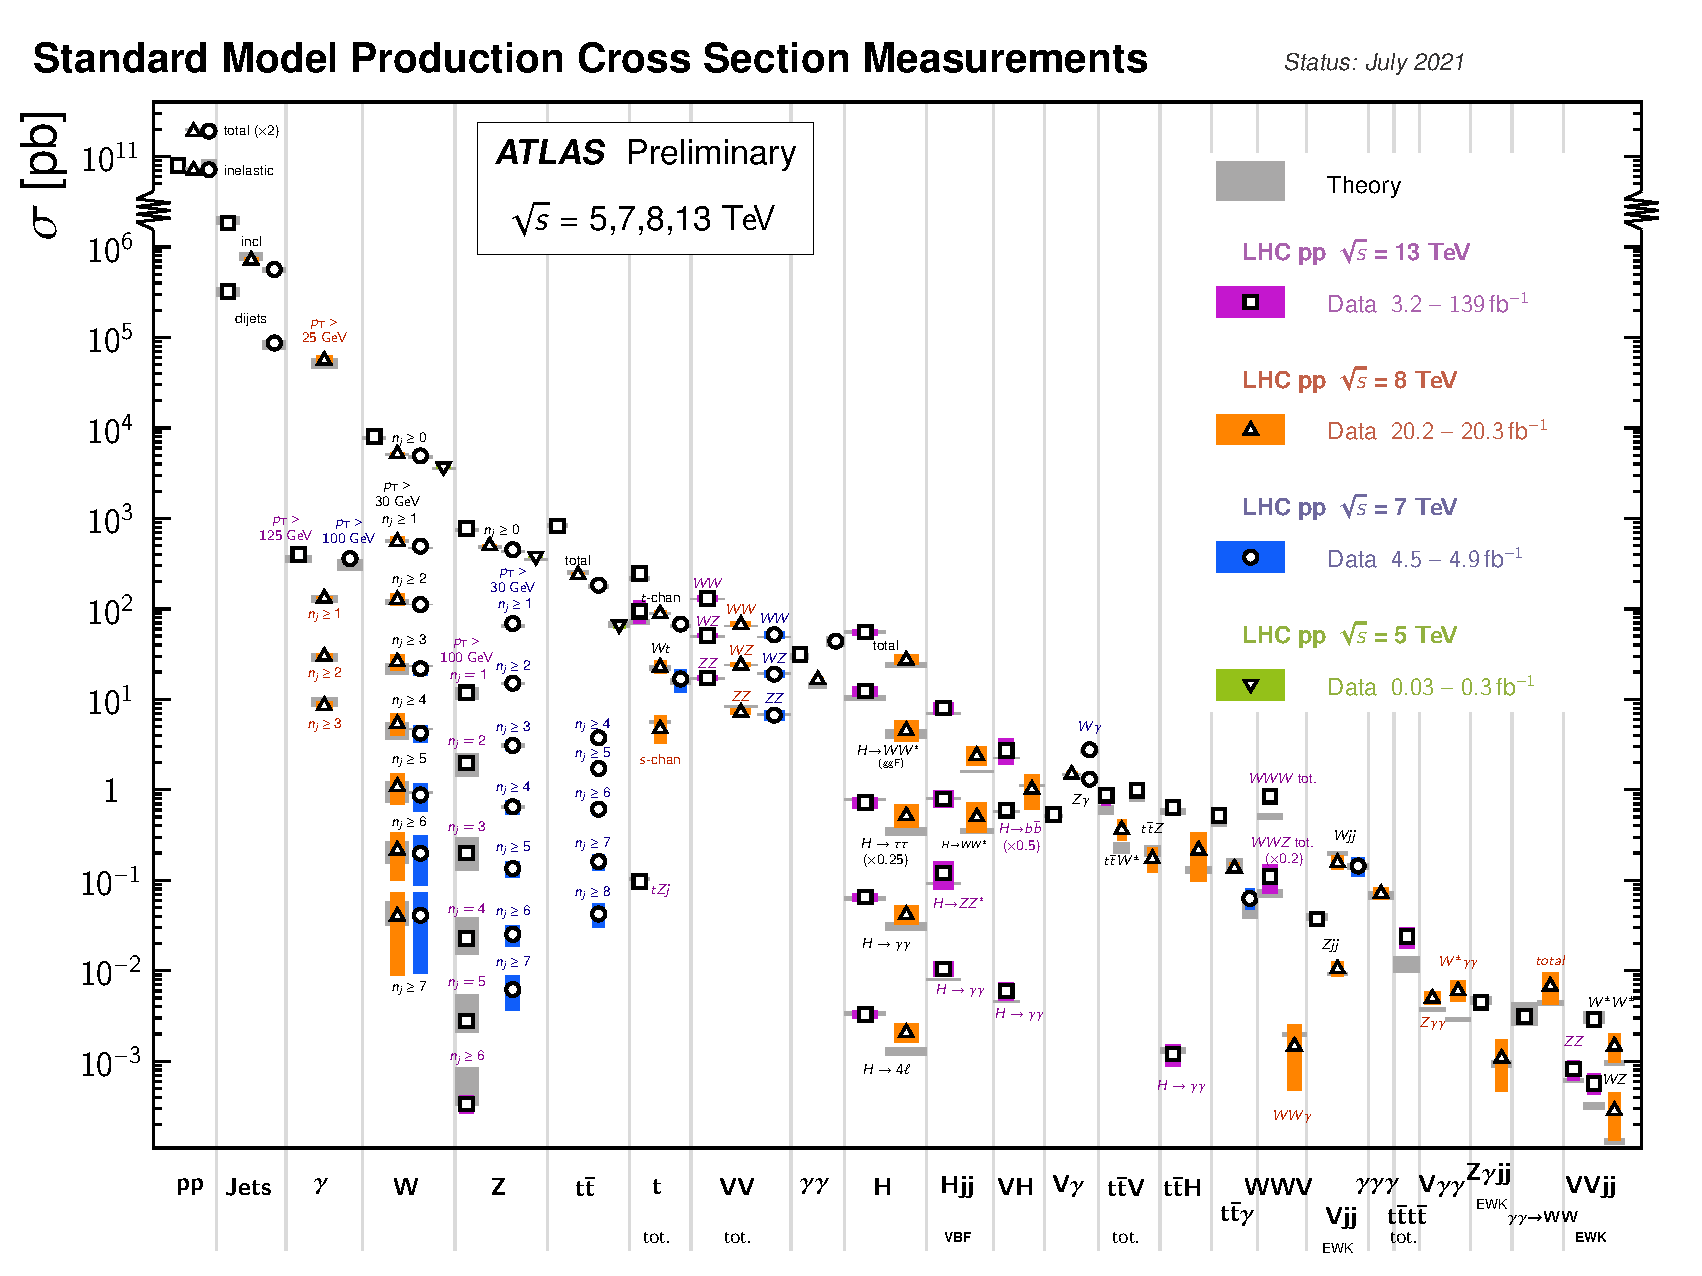
\includegraphics[width=\linewidth]{Assets/Plots/SM/ATLAS_b_SMSummary_FiducialXsect.pdf}
  \caption{Secciones eficaces de producción de los procesos del Modelo Estándar medidas por ATLAS, comparadas con sus estimaciones teóricas \citeonly{ATL-PHYS-PUB-2021-032}.}
  \label{fig:ch1:SM:pp_interactions:cross_sections}
  \setfloatalignment{b}
\end{figure}





\subsection{Limitaciones del Modelo Estándar}

El Modelo Estándar es un triunfo sin precedentes en la carrera por describir las materia e interacciones fundamentales del universo a todas las escalas de energía. Sin embargo, como se ha mencionado en la introducción, se trata de una teoría incompleta. A continuación, describiremos brevemente algunos de los aspectos problemáticos más recurrentes en el SM.

\paragraph{El problema de las jerarquías}

\begin{marginfigure}[3em]
  \centering
  \subfloat[][\label{fig:SM:limitations:higgs_propagator_1-loop:fermion}]{
    \hspace{1mm}%
    \begin{tikzpicture}
      \begin{feynman}
        \vertex (a) {\(H\)};
        \vertex[right=14mm of a] (b);
        \vertex[right=14mm of b] (c);
        \vertex[right=14mm of c] (d) {\(H\)};
        %
        \diagram*{
          (a) -- [scalar] (b), 
          (c) -- [scalar] (d),
          (b) -- [fermion, half left] (c) -- [fermion, half left] (b)
        };
      \end{feynman}
      \node[above right=7.5mm and 5mm of b] (loop_text) {\(f\)};
    \end{tikzpicture}
  }\\
  \subfloat[][\label{fig:SM:limitations:higgs_propagator_1-loop:scalar}]{
    \hspace{1mm}%
    \begin{tikzpicture}
      \begin{feynman}
        \vertex (a) {\(H\)};
        \vertex[right=21mm of a] (b);
        \vertex[right=21mm of b] (c) {\(H\)};
        \vertex[above=14mm of b] (d);
        %
        \diagram*{
          (a) -- [scalar] (b) -- [scalar] (c),
          (b) -- [scalar, half left] (d) -- [scalar, half left] (b)
        };
      \end{feynman}
      \node[above=1mm of d] (loop_text) {\(S\)};
    \end{tikzpicture}
  }
  \caption{Correcciones cuánticas a un loop al propagador del campo de Higgs, originadas en su interacción con fermiones \subref{fig:SM:limitations:higgs_propagator_1-loop:fermion} y escalares \subref{fig:SM:limitations:higgs_propagator_1-loop:scalar} virtuales.}
  \label{fig:SM:limitations:higgs_propagator_1-loop}
\end{marginfigure}

Si se consideran correcciones radiativas al propagador del campo de Higgs, la masa física del bosón de Higgs $m_H$ resulta modificada sobre su masa desnuda $m_{H, \text{bare}}$ como
\[ m_H^2 = m_{H, \text{bare}}^2 + \delta m_H^2. \]
Por ejemplo, mediante interacciones a 1 loop con fermiones virtuales, como se muestra en el diagrama de la \cref{fig:SM:limitations:higgs_propagator_1-loop}, tendremos
\[ \delta m_{H, f}^2 = -\frac{\abs{\lambda_f}^2}{8\pi^2} \left[ \Lambda_{UV}^2 - 3 m_f^2 \log(\frac{\Lambda_{UV}^2}{m_f^2}) + \dots \right], \]
en donde $\lambda_f$ parametriza el acoplamiento del fermión con el Higgs y $\Lambda_{UV}^2$ es el \textit{cut-off} utilizado para regular las divergencias ultravioletas en las integrales de cada loop.

Considerando contribuciones provenientes del quark top, donde $\lambda_f \sim 1$, y suponiendo que el SM es válido hasta la escala de Planck, es decir, $\Lambda_{UV}^2 \sim m_P^2$, entonces las correcciones de la masa resultan $\delta m_H^2 \sim 10^{30}$. Por lo tanto, para obtener una masa del bosón de Higgs de \SI{125}{\GeV}, compatible con las observaciones experimentales, $m_{H, \text{bare}}$ debe ser especificada en menos de una parte en $\sim 10^{12}$. El requerir ajustes extremadamente precisos de los parámetros de la teoría recibe el nombre de \textit{problema de fine-tuning}.

Una forma de evadir este problema consiste en considerar la existencia de otro escalar complejo $S$, de masa $m_S$, que acople con el campo de Higgs con un término $\sim - \lambda_S \Phi^\dagger \Phi S^\dagger S$. Esto produce una corrección de signo contrario en $\Delta m_H^2$, inhibiendo el impacto de las correcciones a órdenes superior del SM. Las extensiones supersimétricas del Modelo Estándar proveen este tipo de partículas, introduciendo una simetría adicional que resulta en un bosón (fermión) super-compañero, para cada fermión (bosón) original del SM~\cite{Haber2018}.


\paragraph{Masa de neutrinos}

Las reacciones nucleares en el interior del sol producen grandes cantidades de neutrinos electrónicos. Sin embargo, los neutrinos solares observados experimentalmente en la tierra se encuentran distribuidos casi homogéneamente entre $\nu_e$, $\nu_\mu$ y $\nu_\tau$~\cite{TheSuper-KamiokandeCollaboration1998}. Este fenómeno, conocido como \textit{oscilación de los neutrinos}, puede ser explicado si se consideran neutrinos masivos, cuyos autoestados de masa no son autoestados de sabor. Para parametrizar las oscilaciones se introduce una nueva matríz de mezcla similar a la matríz CKM, conocida como matríz PMNS (Pontecorvo-Maki-Nakagawa-Sakata).


\paragraph{Materia y energía oscura}

Las observaciones astronómicas de la posición y trayectoria de las estrellas indican que, para que el movimiento rotacional y estructura de las galaxias se ajuste a los modelos de gravedad de la Relatividad General, debería encontrarse una cantidad de materia muy superior a la observada experimentalmente~\cite{Duda2011}. Al no detectarse en forma directa, se supone que este defecto de materia se encontrará compuesto de partículas masivas que no interactuen con el electromagnetismo. Los neutrinos del SM no poseen la masa suficiente para resolver este defecto, por lo que se propone la existencia de una nueva partícula (o familia de partículas), que recibe el nombre de \textit{materia oscura}\sidenote{Ya que no acopla de forma directa con los fotones.}, solo interactuando de forma directa en el SM con el mediador débil $Z^0$.

Los modelos cosmológicos más precisos estiman que la materia fermiónica cargada del SM solo compone un 5\% del universo observable, resultando en un 26\% de materia oscura. Los fotones y neutrinos masivos contribuyen solo un 1\% adicional. Más aún, para modelar la geometría \textit{de-Sitter} del universo en expansión acelerada, se requiere que el restante 68\% de este se encuentre conformado por \textit{energía oscura}. Esta energía, de naturaleza totalmente desconocida, sería la responsable de contraarrestar los efectos de la materia y energía convencional proveyendo una presión negativa, bajo la cual la expansión del universo debería desacelerarse.


\paragraph{Strong-CP}

El Modelo Estándar no establece en sus postulados una conservación de la simetría CP en la interacción fuerte. De hecho, la teoría de QCD provee un término capaz de romper globalmente esta simetría, 
\begin{equation}
  \Lag_{QCD, CP-\text{breaking}} = \theta \frac{\alpha_s}{8\pi} G^{a\mu\nu} \tilde{G}^a_{\mu\nu},
  \label{eq:ch1:SM:limitations:QCD_CP-breaking}
\end{equation}
conocido como \textit{término-$\theta$}, por el parámetro homómino~\cite{Baluni1979}. Sin embargo, a diferencia de la interacción electrodébil, nunca se ha observado evidencia de violación CP en este sector. 

En particular, la presencia de violación CP inducida eventualmente por la existencia de valores no nulos del parámetro $\theta$ de la teoría se encontraría vinculada a un momento dipolar eléctrico en los neutrones~\cite{Crewther1979}. Los resultados experimentales negativos en la búsqueda del momento dipolar del neutrón~\cite{Harris1999} imponen cotas superiores muy estrictas en el valor de $\theta$, y por extensión a la magnitud posible de violación CP en el SM. 

Fijar el parámetro $\theta$ en valores tan pequeños se conoce como problema de \textit{strong-CP}. Algunas teorías que podrían explicar la conservación CP en la interacción fuerte implican la existencia de una nueva partícula pseudoescalar, el axión, de la que hablaremos a continuación.




\section{Extensiones pseudoescalares del Modelo Estándar}

El descubrimiento reciente del bosón de Higgs marcó una nueva era de la física fundamental: no solo representó completar la tabla de partículas predichas por el Modelo Estándar --que estudiamos en la \cref{fig:ch1:SM:particles}--, sino que también ha sido la primera resonancia\sidenote{Se llama resonancia a un pico localizado alrededor de una energía específica de la sección eficáz diferencial en experimentos de scattering.} fundamental escalar detectada experimentalmente. Sin embargo, anticipando el descubrimiento del bosón de Higgs, muchos modelos BSM han incluido otras partículas elementales escalares como parte fundamental de su estructura, como en las extensiones supersimétricas del SM, o los modelos SM ampliados con $N$ dobletes de Higgs (NHDM, \textit{$N$ Higgs Doublet Model}).

En particular, cuando estas extensiones contienen campos escalares complejos, como consecuencia de la ruptura de las simetrías de Gauge, se suelen introducir escalares \textit{CP-odd} (referidos usualmente como \textit{pseudoescalares}) en los espectros de las teorías. Confirmar su existencia resultaría evidencia de física más allá del SM, por lo que los pseudoescalares se encuentran hoy en el centro de varias búsquedas en el LHC.

En las últimas décadas, se ha prestado particular atención a la posibilidad de emplear escalares \textit{CP-odd} como mediadores entre la materia oscura y las partículas del SM, al intentar describir los excesos de rayos gamma difusos en el centro de la galaxia. Estos pseudoescalares suelen ser modelados como \textit{partículas tipo-axiones}, cuya fenomenología será introducida en la siguiente sección, o como bosones \textit{CP-odd} provenientes de la ruptura de simetría del sector de Higgs en el modelo supersimétrico NMSSM (\textit{Next-to-Minimal-Supersymmetric-Standard-Model})\cites[-1em][]{Cheung2014}{Huang2014}.


\subsection{Axion Like Particles}

Los axiones son partículas pseudo-escalares, propuestas por Peccei y Quinn en 1977 como una posible solución al problema \textit{strong-CP}~\cite{Peccei1977,Peccei1977a}. Se introduce una nueva simetría $U(1)$, conocida comunmente como \textit{simetría PQ}, en referencia a los creadores de la teoría, que resulta rota espontáneamente por un campo escalar cargado $\Phi_{PQ}$ que obtiene un vev $v_{PQ} = (f_{PQ} + \phi) e^{i\phi}$. El modo de Goldstone $\phi$ es el axión, una partícula pseudoescalar (impar ante transformaciones $CP$, o \textit{CP-odd}) que hereda una simetría de desplazamiento contínua aproximada $\phi \to \phi + \alpha$, de la simetría PQ original $U(1)$. El axión tiene un acoplamiento anómalo con el $G_{\mu\nu} \tilde{G}^{\mu\nu}$, por medio del que podemos cancelar el efecto del término \eqref{eq:ch1:SM:limitations:QCD_CP-breaking} con una reparametrización $\phi \to \phi' = \phi - \theta$, y un potencial que induzca un mínimo en $\phi' = 0$.

Por convención, el axion normalizado se suele escribir como $a = f_{PQ} \phi$, con una masa dada por $m_a \sim f_{PQ}^{-1}$. La simetría de desplazamiento aproximada de $\phi$ significa que sus acoplamientos con otros campos solo serán en términos de las derivadas $\partial_\mu a$, suprimidos en potencias de $1/f_{PQ}$, restringidas por $f_{PQ} \gg m_{\text{weak}}$~\cite{Powell2016}. En particular, para $f_{PQ} \sim 10^{12} \si{\GeV}$, los axiones pueden ser candidatos a partículas de materia oscura fría ultra-liviana.

Existen muchas modelos BSM que en los límites de bajas energías se reducen a teorías efectivas con simetrías $U(1)$ rotas, también con una simetría de desplazamiento aproximada (por lo que son llamados pseudo-bosones de Goldstone), resultando en campos cuya fenomenología puede ser tratada de una forma análoga a los axiones. Por ejemplo, esto ocurre en abundancia en distintas variedades de teorías de cuerdas, en modelos con Majorones\sidenote[][-3em]{Los Majorones son bosones de Goldstone, denotados $J$, que se proponen como mediadores de la violación $B-L$ (diferencia entre el número bariónico y el número lepónico) en algunas colisiones en altas energías, como $e^- + e^- \to W^- + W^- + J$}, y en modelos con relaxiones\sidenote{Los relaxiones son escalares livianos, propuestos como una solución al problema de las jerarquías, relajando dinámicamente la masa del Higgs con respecto a su elevada masa natural.}.

En todos los casos, las partículas tipo-axiones (ALPs, \textit{Axion-like particles}) son bosones pseudo-escalares, asociados a la ruptura espontánea parcial de estas nuevas simetrías globales $U(1)$, aunque sin la relación entre la masa y los acoplamientos requerida en los axiones. Estas partículas pueden interactuar débilmente con todas las partículas del Modelo Estándar por medio de acoplamientos derivativos, resultando en una amplia variedad de estados finales. Debido a la simetría de desplazamiento aproximada del modo de Goldstone, las ALPs pueden ser muy livianas con respecto a la escala electrodébil, e incluso respecto a la escala de la interacción fuerte. Estas partículas también introducen una solución al problema \textit{strong-CP}. 

Si $C_{\gamma\gamma}/f_a \sim \SI{1}{\TeV^{-1}}$, donde $C_{\gamma\gamma}$ es la constante de acoplamiento de la partícula con un par de fotones, las ALPs podrían proveer una explicación para las discrepancias de las mediciones del factor giromagnético $g-2$ del muón más recientes ($4.2\sigma$~\cite[-9em][]{TheMuong-2Collaboration2021}), respecto a los valores predichos por el SM. Más aún, extensiones BSM con ALPs pueden explicar la aparente violación de universalidad leptónica observada en decaimientos raros de mesones-$B$ por LHCb~\cites[-9em][]{TheLHCbcollaboration2017}[-5em][]{TheLHCbCollaboration2019}[-1em][]{TheLHCbCollaboration2021}, las anomalías en los decaimientos excitados del Berilio (${}^{8*}\text{Be} \to {}^8\text{Be} + e^+ e^-$) y Helio (${}^{4*}\text{He} \to {}^4\text{He} + e^+ e^-$) medidos por la colaboración ATOMKI~\cites[7.5em][]{Krasznahorkay2018}{Krasznahorkay:2019lyl}, y los excesos en el decaimiento del pión neutral $\pi^0 \to e^+ e^-$ observada por KTeV~\cite{Abouzaid2007}.

\begin{figure*}[t]
  \centering
  \subfloat[][\label{fig:ch1:ALP:g-vs-m_a:g_agamma}]{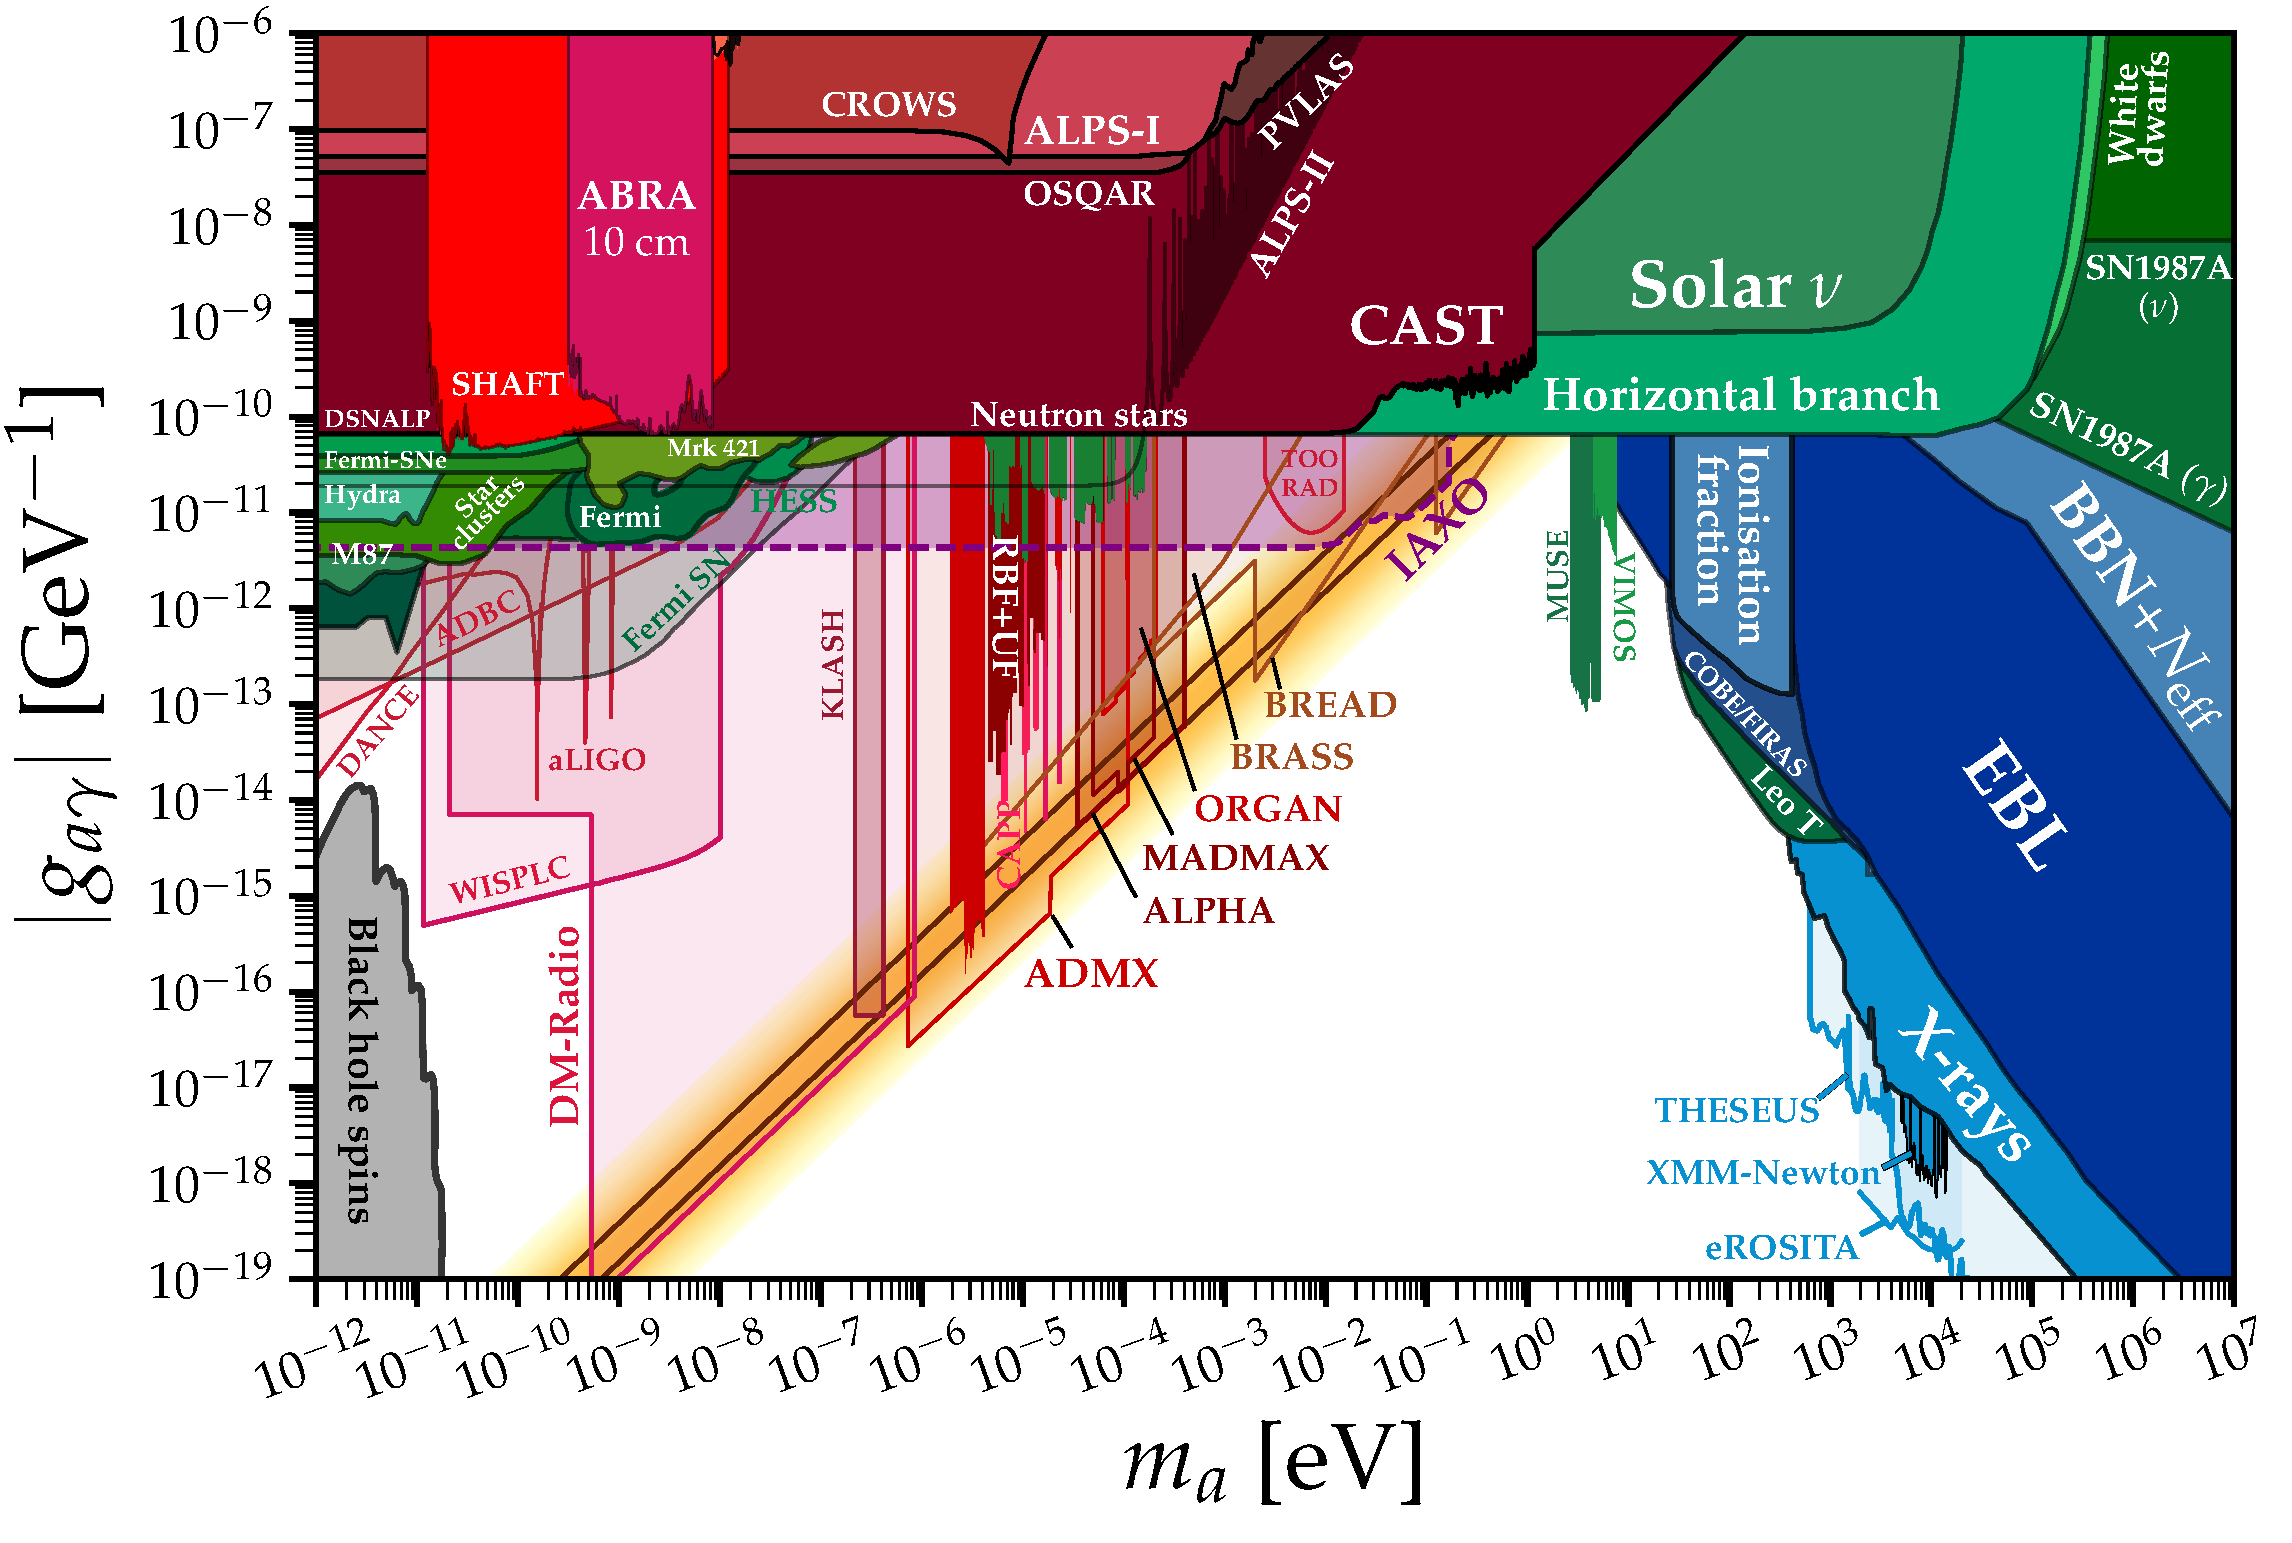
\includegraphics[height=65mm]{Assets/Plots/ALPs/AxionPhoton_with_Projections.pdf}}
  \hfill
  \subfloat[][\label{fig:ch1:ALP:g-vs-m_a:g_ll}]{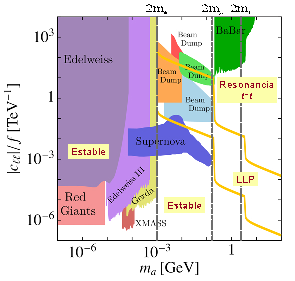
\includegraphics[height=67.5mm]{Assets/Plots/ALPs/Axions_2l.pdf}}

  \caption[][1.5em]{Constantes de acoplamiento en función de la masa $m_a$ de la ALP: $g_{a\gamma} = C_{\gamma\gamma}/f_a$ \subref{fig:ch1:ALP:g-vs-m_a:g_agamma}~\citeonly{OHARE2020}; $C_{\ell\ell}/f_a$ \subref{fig:ch1:ALP:g-vs-m_a:g_ll}~\citeonly{Bauer:2021mvw}. Se muestran los límites teóricos y experimentales establecidos. En \subref{fig:ch1:ALP:g-vs-m_a:g_ll} se detalla la característica experimental de la partícula: estable, de vida larga (LLP) y con resonancias dileptónicas detectables. Se supone $C_{ee} = C_{\mu\mu} = C_{\tau\tau}$.}
  \label{fig:ch1:ALP:g-vs-m_a}
\end{figure*}

En las últimas dos décadas, las ALPs han cobrado particular relevancia como mediadores entre la materia oscura y los fotones del SM, pudiendo explicar los escesos de radiación gamma difusa en el centro galáctico~\cite{Hooper2011,Abazajian2012,Daylan2016}, en el contexto de modelos de \textit{Coy dark matter}~\cite{Bhm2014,Hektor2014}. En estos modelos, la materia oscura es modelada por partículas fermiónicas, interactuando con el SM por medio del intercambio de una ALP mediadora muy liviana.

Los modelos de ALPs de orígen astrofísico son válidos a lo largo de muchos órdenes de magnitud de masas y constantes de acoplamiento. Por ejemplo, los límites establecidos de la constante de acoplamiento de la interacción entre la ALP y los fotones, se exhiben en la \cref{fig:ch1:ALP:g-vs-m_a:g_agamma}.

Las ALP pueden ser tratadas convenientemente utilizando un lagrangiano efectivo suponiendo violación CP y MFV (\textit{Minimal Flavour Violation})~\cite{DAmbrosio2002}, que en dimensión de masa $d \leq 5$, al órden más pequeño en el parámetro de escala de ruptura de simetría $f_a$, puede expresarse como
\begin{align*}
  \Lag_{ALP}^{d \leq 5} &= \inv{2} \partial_\mu a \partial^\mu a - \frac{m_a^2}{2} a^2 \\*
             &\quad\quad - \frac{C_{\tilde{B}}}{f_a} B_{\mu\nu} \tilde{B}^{\mu\nu} a - \frac{C_{\tilde{W}}}{f_a} W_{\mu\nu} \tilde{W}^{\mu\nu} a - \frac{C_{\tilde{G}}}{f_a} G_{\mu\nu} \tilde{G}^{\mu\nu} a \\*
             &\quad\quad + \sum_{i = u, d, e, \dots} \frac{C_f}{f_a} \bigg[ \bar{f}_i \gamma^\mu \ \bigg( \underbrace{\frac{\mathds{1} + \gamma^5}{2}}_{P_R} \bigg) \ f_i \bigg] \partial^\mu a + \mathcal{O}( f_a^{-2} ),
\end{align*}
implicando $6 + m_a$ parámetros independientes. Si bien este lagrangiano presenta términos de interacción con casi todas las partículas del SM\sidenote{El acoplamiento con el bosón de Higgs se hace presente en interacción de dimensiones superiores, siendo los primeros no nulos en $d = 6$ ($\sim haa$) y $d = 7$ ($\sim hZa$).}, los vértices de mayor interés a orden dominante serán los que relacionen a la ALP $a$ con los Bosones de Gauge y los fermiones, como podemos observar en la \cref{fig:ch1:ALP:vertices}. Al suponer MFV, estas partículas tendrán interacciones dominantes con fermiones de la tercera generación: quarks $t$, $b$ y leptones~$\tau$~\cite{Bauer2017,Bauer2017a,Bauer2019}.

Los acoplamientos a nivel árbol con un par $\gamma\gamma$ y $Z\gamma$ serían los principales responsables de la producción de rayos gamma difusos en el centro de la galaxia. Además, estos permiten realizar búsquedas directas de ALPs en colisiones hadrónicas de altas energías --como las realizadas en el LHC-- estudiando la dispersión de dos fotones, o la producción de ALPs estables junto a un único fotón, $Z \to a\gamma$~\cite{Schmieden2021,TheATLASCollaboration2021}. Los vértices de interacción de las ALPs con fermiones son proporcionales a la masa del fermión. Por lo tanto, serán dominantes los acoplamientos con los fermiones de tercera generación, resultando también de interés la producción de ALPs en colisionadores en asociación a un par de quarks top ($t\bar{t}a$) y bottom ($b\bar{b}a$), y los canales de decaimiento $a \to b\bar{b}$ y $a \to \tau^-\tau^+$. Esto brinda acceso a ALPs más pesadas a las accesibles en estudios astronómicos, con $m_a \gtrsim \SI{10}{\GeV}$. 

Dependiendo de la masa y la constante de acoplamiento, son accesibles distintos regímenes experimentales, como podemos observar en la \cref{fig:ch1:ALP:g-vs-m_a:g_ll} para el decaimiento dileptónico. Si la constante de acoplamiento es muy pequeña, o la $m_a$ es inferior a la masa de las partículas del estado final (en el caso que se trate de un decaimiento a partículas masivas), la ALP se dice estable. Por lo tanto, esta escapará al detector, pudiendo solo ser observada como un faltante de momento al aplicar los teoremas de conservación. Por el contrario, si la interacción es lo suficientemente fuerte, se habilita la posibilidad de un decaimiento resonante. El caso medio resulta en partículas inestables, pero de una larga vida media (LLP, \textit{Long Lived Particles}), por lo que su vértice de decaimiento se encontrará desplazado del vértice de su creación. En particular, el decaimiento resonante a dos leptones pesados $a \to \mu^-\mu^+/\tau^-\tau^+$ se encuentra en una región mayormente inexplorada del espacio de parámetros.

\begin{marginfigure}
  \centering
  \begin{align*}
    &\feynmandiagram [small, inline=(vert.base), horizontal=a to vert] {
      a [particle=\(a\)] -- [scalar] vert,
      f1 [particle=\( \gamma \)] -- [photon] vert -- [photon] f2 [particle=\( \gamma \)],
    };
    \quad
    \propto (c_\theta^2 C_{\tilde{B}} + s_\theta^2 C_{\tilde{W}}),\\
    %
    &\feynmandiagram [small, inline=(vert.base), horizontal=a to vert] {
      a [particle=\(a\)] -- [scalar] vert,
      f1 [particle=\( Z^0 \)] -- [boson] vert -- [boson] f2 [particle=\( Z^0 \)],
    };
    \quad
    \propto (c_\theta^2 C_{\tilde{W}} + s_\theta^2 C_{\tilde{B}}),\\
    %
    &\feynmandiagram [small, inline=(vert.base), horizontal=a to vert] {
      a [particle=\(a\)] -- [scalar] vert,
      f1 [particle=\( Z^0 \)] -- [boson] vert -- [photon] f2 [particle=\( \gamma \)],
    };
    \quad
    \propto s_\theta c_\theta (C_{\tilde{W}} - C_{\tilde{B}}),\\
    %
    &\feynmandiagram [small, inline=(vert.base), horizontal=a to vert] {
      a [particle=\(a\)] -- [scalar] vert,
      f1 [particle=\( W^+ \)] -- [boson] vert -- [boson] f2 [particle=\( W^- \)],
    };
    \quad
    \propto C_{\tilde{W}} \hspace{0.7em} +(aWWZ/\gamma),\\
    %
    &\feynmandiagram [small, inline=(vert.base), horizontal=a to vert] {
      a [particle=\(a\)] -- [scalar] vert,
      f1 [particle=\( G \)] -- [gluon] vert -- [gluon] f2 [particle=\( G \)],
    };
    \quad
    \propto C_{\tilde{G}} \quad\quad +(aGGG),\\
    %
    &\feynmandiagram [small, inline=(vert.base), horizontal=a to vert] {
      a [particle=\(a\)] -- [scalar] vert,
      f1 [particle=\( f_i \)] -- [anti fermion] vert -- [anti fermion] f2 [particle=\( \bar{f}_i \)],
    };
    \quad
    \propto C_f m_{f_i}.
  \end{align*}
  \caption[Vértices de interacción, de dimensión $d \leq 5$, de mayor interés en teorías BSM con ALP.]{Vértices de interacción, de dimensión $d \leq 5$, de mayor interés en teorías BSM con ALPs. $s_\theta$ y $c_\theta$ son el seno y coseno del ángulo de Weinberg $\theta_w$ respectivamente.}
  \label{fig:ch1:ALP:vertices}
\end{marginfigure}


\subsection{Búsqueda de bosones pseudoescalares en el LHC}

En contraste al paradigma ampliamente aceptado que sugiere que las nuevas partículas fundamentales tienen que ser más pesadas que los actuales constituyentes del Modelo Estándar, con $m_{BSM} \gtrsim \mathcal{O}(\SI{1}{\TeV})$, las masas de bosones pseudoesclares no se encuentran casi restringidas por búsquedas directas, como hemos mencionado en el caso particular de las ALPs.

Como las interacciones entre los bosones de gauge y los escalares \textit{CP-odd} solo pueden ser inducidas por operadores de mayor dimensión ($\sim a \epsilon_{\mu\nu\rho\sigma} V^{\mu\nu} V^{\rho\sigma}$), los límites establecidos por el LEP son particularmente débiles~\citeonly{Bauer:2021mvw,Casolino2015}. Las mayores sensibilidades en colisionadores provienen de producciones asociadas a los quarks $t$ o $b$, al imponer MFV en muchos de estos modelos. Existen algunos límites provenientes de la física de sabores, pero estos son nuevamente muy débiles si $m_a \gtrsim \SI{5}{\GeV}$~\citeonly{Dolan2015}. Por lo tanto, para detectar la existencia de partículas pseudoescalares en la escala de la interacción electrodébil en el LHC, la mejor estrategia consiste en realizar nuevas búsquedas directas.

Si bien podemos encontrar bosones pseudoescalares en muchos modelos, como hemos detallado en las secciones anteriores, resulta útil proponer un modelo de señal BSM que resulte independiente de los detalles específicos de cada teoría, solo reteniendo las principales características de los modos de producción y decaimiento.




{ % I have to remove the "Global" \smallcapslsstyle{50}, because it ruins math text 
\titleformat{\subsection}%
  [hang]% shape
  {\normalfont\color{darkgray}\Large}% format applied to label+text
  {\large\smallcapslsstyle{50}{\thesubsection}}% label
  {1em}% horizontal separation between label and title body
  {}% before the title body
  []% after the title body
\subsection{{\lsstyle\scshape\MakeTextLowercase{Modelo de señal}} \texorpdfstring{$t\bar{t}X$, $X \to \tau\tau$}{ttX, X -> tautau}}
} \label{sec:ch1:ttX_phenomenology:signal}

Siguiendo los lineamientos y las motivaciones teóricas enunciadas, en el presente análisis se procede a la búsqueda de una resonancia liviana pseudoescalar $X$, de masa $m_X < \SI{60}{\GeV}$, producida en asociación con un par de quarks top, y con un canal de decaimiento a un par de leptones taus. El diagrama de Feynman de este proceso se exhibe en la \cref{fig:ch1:pseudoscalars:ttX:diagram}.

\begin{figure}[t]
  \centering
  \resizebox{0.7\linewidth}{!}{\ttXdiagram[small]}
  \caption{Diagrama de Feynman del proceso de señal $t\bar{t}(X \to \tau\tau)$ buscado en el presente análisis.}
  \label{fig:ch1:pseudoscalars:ttX:diagram}
  \setfloatalignment{b}
\end{figure}

El par de quarks $t\bar{t}$ se considera en el modo de decaimiento semi-leptónico. En este canal, uno de los quarks $t$ decae leptónicamente a $t \to b + (W \to \ell + \nu_\ell)$, mientras que el otro quark decae hadrónicamente como $t \to b + (W \to q + \bar{q})$, produciendo dos jets adicionales. De esta manera, se dispone de un leptón que puede ser utilizado como \textit{trigger} de los eventos de señal. La presencia de al menos 2 quarks $b$ en todos los eventos permite también suprimir eventos de fondo.

Al tener masa elevada, los leptones \ttau decaen después de una vida media de solo $\tau \sim \SI{2.9e-13}{\second}$~\cite{Zyla2020}. Debido a la longitud propia $c\tau \sim \SI{87}{\micro\meter}$, la mayoría de los decaimientos de taus se dan en extrema proximidad del vértice de producción, por lo que solo podrán ser estudiados experimentalmente mediante los productos de su decaimiento.

\begin{marginfigure}
  \feynmandiagram [layered layout, horizontal=a to b] {
    a [particle=\(\tau^{-}\)] -- [fermion] b -- [fermion] f1 [particle=\(\nu_{\tau}\)],
    b -- [boson, edge label'=\(W^{-}\)] c,
    c -- [fermion] f2 [particle=\(\text{$e^-$, $\mu^-$, $d$}\)],
    c -- [anti fermion] f3 [particle=\(\text{$\bar{\nu}_e$, $\bar{\nu}_\mu$, $\bar{u}$}\)],
  };
  \caption{Diagrama de Feynman del decaimiento de un leptón $\tau$, en el modo de decaimiento leptónico (a un par $e\bar{\nu}_e$ o $\mu\bar{\nu}_\mu$) y hadrónico (decayendo a un par de quarks $d\bar{u}$).}
  \label{fig:ch1:pseudoscalars:tau_decay}
\end{marginfigure}

Los leptones $\tau$ decaen el 35.2\% de las veces en un modo leptónico, dado por $\tau^- \to e^- \bar{\nu}_e \nu_\tau$ y $\tau^- \to \mu^- \bar{\nu}_\mu \nu_\tau$, como podemos observar en el diagrama de la \cref{fig:ch1:pseudoscalars:tau_decay}. La interacción de los neutrinos con los detectores es muy improbable, por lo que solo son observadas las partículas cargadas. Por lo tanto, el decaimiento leptónico de los taus resulta difícil de distinguir con respecto a electrones y muones de producción directa (\textit{prompt}).

En el modo de decaimiento hadrónico, con un \textit{branching ratio} de 64.6\%, los taus decaen a un neutrino $\nu_\tau$ y uno o más hadrones cargados. En este caso, las trazas de los hadrones cargados y sus señales en los calorímetros pueden ser detectadas e identificadas con mayor precisión, por lo que se estudiará solo este canal de decaimiento en la presente búsqueda. Los productos finales del decaimiento suelen ser al menos un mesón cargado, como un pión $\pi^\pm$ o un kaón $K^\pm$, y posiblemente mesones neutros, como $\pi^0$ y $K^0$. En general, el decaimiento a una única partícula cargada es denominado \textit{1-prong}, con un \textit{branching ratio} de $50.0\%$ en los decaimientos hadrónicos, mientras que el decaimiento a 3 partículas cargadas, con una probabilidad de $14.6\%$, recibe el nombre de \textit{3-prong}.

Existen decaimientos exóticos a 3 leptones cargados, un hadrón cargado y dos leptones, o 5 hadrones cargados, aunque estos poseen una probabilidad despreciable, inferior a $10^{-4}\%$, por lo que serán ignorados.

Para modelar los procesos de señal, utilizaremos una extensión del sector de Higgs del SM, conocida como 2HDM (\textit{2 Higgs Doublet Model})~\cite{Degrande2015a,Jurciukonis2019}. Una breve descripción de este modelo se encuentra en el \cref{ap:ap1}.

\vspace{1em}
\subsubsection{Topología del evento de señal}

Como veremos en el \cref{chap:ch2}, en física de altas energías se suele adoptar un sistema de coordenadas cilíndrico $(z,\phi,\eta)$, donde $\eta$ se encuentra referida al ángulo polar $\theta$ como $\eta = -log(\tan(\theta/2))$. Esto permite definir una medida de distancia angular entre cualquier par de puntos $\Delta R = \sqrt{\Delta\phi^2 + \Delta\eta^2}$.

En general, puede demostrarse~\cite[-2em][]{Han2017} que para un objeto que decae en dos partículas de menor masa, la separación angular de los productos de decaimiento se encuentra dada por
\[ \Delta R_{1,2} \approx \frac{2m}{p_T} \label{eq:ch1:ditau:angular_sep}, \]
donde $m$ y $p_T$ son la masa y el momento transverso de la partícula madre. El régimen $m \gg p_T$, donde los productos de decaimiento se encuentran claramente separados, recibe el nombre de \textit{resolved} (resuelto), mientras que si $p_T \gg m$ se lo llama \textit{boosted} (\textit{boosteado})

\begin{marginfigure}
  \centering
  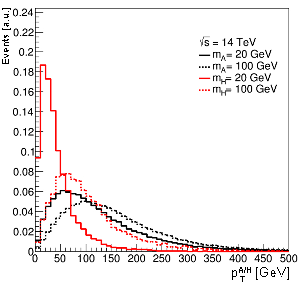
\includegraphics[width=\linewidth]{Assets/Plots/ttX/h_A-H_pT.pdf}
  \caption{Momento en el plano transverso $p_T$ de una partícula escalar $H$ (rojo) y pseudoescalar $A$ (negro), producida en asociación con un par de quarks $t\bar{t}$ en una colisión protón-protón con energía de centro de masa $\sqrt{s} = \SI{14}{\TeV}$.}
  \label{fig:ch1:pseudoscalars:A-vs-H_pT}
\end{marginfigure}

\begin{marginfigure}
  \centering
  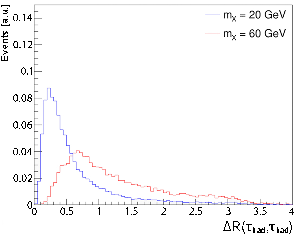
\includegraphics[width=\linewidth]{Assets/Plots/ttX/h_A_DeltaR.pdf}
  \caption{Separación angular $\Delta R$ entre el par de \ttaus producidos por el decaimiento de una partícula pseudoescalar de bajas masas.}
  \label{fig:ch1:pseudoscalars:A_DeltaR}
\end{marginfigure}

En los eventos de señal $t\bar{t}X$, debido a la conservación de la energía en la interacción, la reducida masa de la resonancia buscada ($\lesssim \SI{60}{\GeV}$) respecto a los quarks top ($\SI{173}{\GeV}$) resulta en una elevada magnitud de la fracción $p_{T, X}/m_X$.

Más aún, una de las consecuencias del cambio en la interacción entre los quarks top y el bosón pseudoescalar, respecto a un caso análogo con una partícula escalar \textit{CP-even}, es un espectro de momentos sustancialmente desplazado a energías superiores. Podemos observar este fenómeno en la \cref{fig:ch1:pseudoscalars:A-vs-H_pT}, que contiene las distribuciones simuladas del momento en el plano transverso de una colisión protón-protón de ambas partículas.

En los eventos de señal de interés, esto resulta en una muy pequeña separación angular $\Delta R$ entre los \ttaus, como podemos observar en la \cref{fig:ch1:pseudoscalars:A_DeltaR}. Esto representa un gran desafío en el análisis experimental, ya que impide la correcta reconstrucción e identificación de los \thads en los detectores, requiriendo la implementación de nuevas técnicas de análisis que desarrollaremos en la \cref{sec:ch3:ditaus}. La eficiencia de estos métodos determinará el rango de masas total abarcado en la búsqueda.


\cleardoublepage{}